\documentclass{book}
\usepackage{blindtext}
\usepackage[T1]{fontenc}
\usepackage[polish]{babel}
\usepackage[utf8]{inputenc}
\usepackage{listings}
\usepackage{graphicx}
\usepackage{float}
\usepackage{multirow}
\usepackage{hyperref}
\usepackage[table,xcdraw]{xcolor}
\usepackage{textcomp}
\usepackage{pdfpages}
\usepackage{float}
\floatstyle{plaintop}
\restylefloat{table}
\graphicspath{ {./Wykresy/} }


\title{Analiza wpływu zastosowania wybranych technik przygotowania danych do analizy, na jakość analizy danych}
\author{Dariusz Litwiński}
\date{\today}

\renewcommand\lstlistingname{Przykład}

\begin{document}

\includepdf{DL_Strona_tytulowa.pdf}

\tableofcontents



\chapter*{Wstęp}

\section*{Wprowadzenie do problemu}
Analiza danych to proces, 
w którym przekształcamy surowe dane w wiedzę i 
wnioski, dzięki którym jesteśmy w stanie podejmować lepsze decyzje \cite{data_analysis_def}.
Im dokładniejsza analiza, tym trafniejsze decyzje będziemy w 
stanie podjąć na jej podstawie, dlatego powinno się ten proces wielokrotnie powtarzać, 
za każdym razem próbując uzyskać lepsze rezultaty. Skupiając się na przygotowaniu danych można uzyskać 
znaczącą poprawę wyników, ponieważ dane bardzo często zawierają wartości brakujące, nieodpowiednio zakodowane, bądź
można uzyskać dodatkowe informacje poprzed odopowiednie ich spreparowanie.
Decyzja jakie środki przygotowania danych zastosować bywa trudna i wymaga czasu oraz zbadania zbioru danych, a także
bardzo często nie daje aż tak wymiernych rezultatów jakich się spodziewamy.

\section*{Cel pracy}
Celem pracy jest sprawdzenie, jak poszczególne metody przygotowania danych
wpływają na jakość analizy danych, konkretnie modelowania klasyfikatorów. Przeprowadzono 
eksperymenty z użyciem wielu metod przygotowania danych, a następnie porównano trafność klasyfikacji 
względem klasyfikatora bez przygotowania danych. Za brak przygotowania danych uznaje się usunięcie 
wszystkich rekordów z brakującymi wartościami oraz wszystkich kolumn nieliczbowych.
Rozpoczynając prace postawiono hipotezę, że najlepszym sposobem na przygotowanie danych jest dogłębne 
ich zrozumienie, a następnie dostosowanie do nich użytych metod, jak i rówież fakt, że jakiekoliwek przygotowanie 
danych powinno wpłynąć pozytywnie na jakość analizy danych.

\section*{Zawartość pracy}
W pracy krótko przedstawiono problem analizy danych, wyliczono 
typy metod przygotowania danych, opisano wykonane eksperymenty, 
zarówno środowisko w jakim je przeprowadzono, jak i to na czym polegały.
Ostatnią część pracy stanowią wyniki eksperymentów wraz z ich podsumowaniem

\chapter{Problem Analizy Danych}



W poniższym rozdziale wymieniono oraz opisano fazy procesu analizy danych, wprowadzono
pojęcie jakości danych oraz omówiono problemy jakie mogą wystąpić przy pracy z danymi

\subsection*{Pozyskiwanie: gromadzenie danych}
Zanim analiza danych będzie możliwa należy pozyskać dane, 
jest to istotna cześć procesu, ponieważ to od niej zależy to, 
jak trafne wnioski będziemy mogli wysnuć na późniejszych etapach.
Bardzo ważne jest to, jak dużą ilość danych uda nam się zebrać, a także jak dokładne one będą.
Możemy pozyskiwać dane z różnorakich źródeł, na przykład: 
\begin{itemize}
    \item Zapisywać wartości zbierane przez czujniki \cite{data_from_sensors}
    \item Korzystać z ankiet zebranych wśród danej populacji \cite{data_from_questionaire}
    \item Zbierać dane o zachowaniach użytkowników w trakcie korzystania ze strony internetowej \cite{data_from_behavior}
    \item Wykorzystywać dane statystyczne/historyczne \cite{data_from_statistics}
  \end{itemize}
Jesteśmy w tej kwestii ograniczeni jedynie przez dziedzinę, w jakiej przeprowadzamy analizę danych
Istotną kwestią jest również to, w jakim formacie są 
przechowywane dane. Może okazać się, że pierwszym etapem przetwarzania danych 
będzie odpowiednie ich sformatowanie, bądź nawet ich cyfryzacja, jeśli były 
by przechowywane w formie fizycznej, na przykład jako papierowe archiwa


\subsection*{Przygotowanie: przetwarzanie danych}
Aby móc w pełni korzystać ze zgromadzonych danych, 
należy je przygotować, odpowiednio sformatować. 
Poza przygotowaniem odpowiedniego formatu danych, 
możemy wyróżnić następujące sposoby na przygotowanie danych do analizy:
\begin{itemize}
    \item Wypełnienie brakujących wartości 
    \item Standaryzacja danych liczbowych
    \item Kodowanie wartości kategorycznych jako liczbowe
  \end{itemize}
Dzięki wykorzystaniu powyższych sposobów możemy znacznie zwiększyć jakość analizy danych, 
a co za tym idzie wnioski do których dojdziemy w trakcie procesu będą 
trafniejsze i przyniosą lepsze rezultaty


\subsection*{Analiza: modelowanie danych}
Mając do dyspozycji przygotowane dane możemy przejść do ich właściwej analizy, 
na podstawie której tworzymy modele, klasyfikatory \cite{classifiers}, systemy rekomendacji 
\cite{recomendation_systems}, dokonujemy klasteryzacji \cite{clustering}. 
Najczęsciej nie tworzymy ich od zera, a wspomagamy się dostępnymi bibliotekami, które zawierają 
najpopularniejsze algorytmy. Zdarza się, że nie jesteśmy zadowoleni z wyników, jakie przynosi 
wykorzystanie stworzonych modeli, bądź chcielibyśmy dokonać dalszej optymalizacji czasowej, 
w takim przypadku możemy rozważyć dodatkowe przygotowanie danych, aby uzyskać pożądany efekt.
Po dobrze przeprowadzonej analizie, jesteśmy w stanie 
wykorzystać stworzone na tym etapie narzędzia do rozwiązywania rzeczywistych problemów.

\subsection*{Działanie: podejmowanie decyzji}
Mając gotowe narzędzia będące wynikiem modelowania danych, możemy je wykorzystać aby podjąć 
konkretne decyzje w prawdziwym świecie: Wykorzystać stworzony 
klasyfikator w diagnostyce chorób, wdrożyć system rekomendacji 
na naszej stronie internetowej, wykorzystać stworzone klastry danych do kategoryzacji klientów. 
Każdy z przedstawionych problemów wymaga eksperckiej wiedzy oraz ogromnego doświadczenia, 
a dzięki analizie danych możemy znacznie usprawnić ich rozwiązywanie.

\section{Jakość Danych}
Jakość danych jest oceniana na podstawie wielu kryteriów, zależnych od źródła informacji\cite{data_quality}:
\begin{itemize}
    \item Kompletność - ilość danych która jest kompletna bądź zdatna do użycia. Jeśli duża 
    część danych jest niekompletna, może to prowadzić do stronniczej bądź nawet omylnej analizy. 
    \item Unikalność - jaka część z zestawu danych się powtarza, 
    dla przykładu zestaw danych zawierających dane o klientach 
    powinien każdemu z nich przypisać unikalny numer identyfikacyjny
    \item Ważność - To kryterium mówi o tym czy zebrane dane są w odpowiednim formacie
    \item Aktualność - W zależności od dziedziny którą się zajmujemy, dane mogą tracić na aktualności wraz 
    z upływem czasu, przez na przykład postęp w danej 
    dziedzinie bądź zmieniające się warunki
    \item Dokładność - poprawność danych w oparciu o ustalone "źródło prawdy". 
    Jako, że może istnieć wiele źródeł tych samych danych, 
    należy ustalić nadrzędne źródło danych, pozostałe 
    zaś mogą potwierdzać dokładność tego pierwszego.
    \item Stałość - kryterium służące do porównywania danych z dwóch zestawów danych. 
    Używanie różnych źródeł do szukania stałych trendów w danych. 
    Dzięki temu wnioski pojawiające się w trakcie analizy mogą być 
    traktowane z większym zaufaniem, jako że tworzone są na podstawie wielu niezależnych zestawów danych.
    \item Dopasowanie do celu - to kryterium pozwala nam zapewnić fakt, 
    że dane które są zbierane posłużą nam do rozwiązania problemu, jaki przed nami stoi
  \end{itemize}

\section{Problemy z Danymi}

Bardzo często zebrane dane nie nadają się bezpośrednio do pracy z nimi. 
Należy najpierw wykonać szereg operacji aby pozbyć się następujących 
problemów:   
\subsection{Brakujące wartości}
W danych mogą występować brakujące wartości, na przykład czujniki 
mogą różnić się między sobą ilością pobieranych parametrów, 
ankietowani mogą pozostawić niektóre pytania bez odpowiedzi. 
Brakujące wartości stanowią poważny problem, ponieważ model nie 
potrafi ich jednoznacznie zinterpretować, dlatego w trakcie 
przygotowania danych musimy podjąć decyzję, czy usunąć rekordy z 
brakującymi wartościami, przez co możemy znacznie zmniejszyć 
liczebność zbioru danych. Alternatywnym podejściem jest wypełnienie 
brakujących wartości. W miejsce braku może być wstawiona średnia, 
minimum, maksimum, lub też inna arbitralnie wybrana wartość. 
Pozornie wartości wstawiane w puste miejsca są kompletnie arbitralne, 
jednak bardzo często takie podejście skutkuje najlepszymi rezultatami, 
pod warunkiem że dobierzemy odpowiednią wartość do wstawiania. \cite{missing_values}
\subsection{Wartości odstające}
W niektórych przypadkach w danych mogą pojawić się takie wartości, 
które wyraźnie odstają od reszty i nie wnoszą sobą zbyt wiele 
informacji w kontekście analizy danych. Co więcej, mogą one 
zaciemniać pozostałą część danych, maskując trendy bądź prowadząc 
do błędnych wniosków. Dlatego najlepszym podejściem jest wykrywanie 
oraz usuwanie wartości, które możemy uznać za odstające. 
Istnieją algorytmy pozwalające nam na odrzucenie wartości odstających. \cite{outlier_detection}
\subsection{Kolumny kategoryczne}
Wiele z modeli może pracować jedynie na wartościach liczbowych, 
podczas kiedy w zbiorach danych możemy znaleźć nie tylko takie wartości, 
ale również kategoryczne. Rezygnując z analizy tych danych tracilibyśmy 
wiedzę, jaką można z nich pozyskać. Nie jest to jednak konieczne, 
gdyż istnieją sposoby, aby zamienić te dane na postać liczbową za 
pomocą kodowania \cite{enconding}



\chapter{Metody Przygotowania Danych}
Istnieje kilka najczęściej używanych metod przygotowania danych, 
które dzielą się na następujące grupy:

\subsection*{Uzupełnianie brakujących wartości}
Najczęściej brakujące wartości w zbiorach danych uzupełnia się średnią 
lub najczęściej występującą wartością, jednak może zdarzyć się tak, 
że najlepszym rozwiązaniem jest uzupełnienie braków minimum, maksimum, 
zerem bądź inną arbitralnie wybraną wartością
\subsection*{Wykrywanie wartości odstających}
Do wykrywania wartości odstających możemy wykorzystać manualne metody, 
ale również i algorytmy, które wykryją te wartości za nas. 
Do manualnych metod możemy zaliczyć: Wykrywanie za pomocą rozkładu 
normalnego, Z-score, IQR, wykrywanie za pomocą percentyli. 
Natomiast spośród automatycznych metod mamy do dyspozycji między innymi 
Las Izolacji lub Local Outlier Factor
\subsection*{Kodowanie wartości kategorycznych}
Jeżeli znamy zależności między klasami i możemy je uporządkować, 
wtedy jesteśmy w stanie dokonać kodowania ręcznie, na przykład 
najmniejszą wartość dla edukacji podstawowej, a najwyższą dla 
edukacji wyższej. Natomiast jeżeli nie znamy tych zależności, 
możemy wykorzystać LabelEncoder, jednak on ponumeruje klasy w 
kolejności alfabetycnzej, co nie zawsze jest pożądanym rezultatem. 
Innym podejściem jest One-Hot Encoding\cite{one_hot_encoding}, który dla każdej z klas 
tworzy osobną kolumnę z wartością logiczną opisującą, czy dany 
rekord należy do tej klasy. Powoduje to wygenerowanie sporej 
ilości kolumn, jednak mamy wtedy pewność, że nie stworzymy 
nowych zależności między klasami
\subsection*{Standaryzacja}
Standaryzacja jest procesem, po zakończeniu którego zmienna 
ma średnią wartość oczekiwaną zero oraz odchylenie standardowe 
równe jeden, dzięki czemu zyskujemy większą przejrzystość w 
jej analizie. Bardziej wyraźne są skupienia wokół konkretnych 
wartości, jednak należy zadbać o to, aby przed standaryzacją 
pozbyć się wartości odstających, gdyż będą one miały negatywny 
wpływ na zmienną po standaryzacji



\chapter{Środowisko wykonawcze}

W poniższym rozdziale przedstawione zostało środowisko wykonawcze, 
w jakim przeprowadzono eksperymenty, a także opisano zbiory danych, 
na których je przeprowadzono
\subsection*{Specyfikacja sprzetowa, system i środowisko}
Sprzęt: Laptop wyposażony w procesor Intel Core i5-1135G7 
(2.4Ghz) ze zintegrowaną grafiką oraz 16GB pamięci RAM
System operacyjny: Windows 10 Education
Menadżer środowisk: Anaconda Navigator
Python: 3.9.12
Edytor kodu: Visual Studio Code z dodatkami do edycji plików w 
formacie Jupyter notebook
\section{Zbiory danych}
Zbiory na których będziemy sprawdzać wpływ przygotowania danych 
są zbiorami do klasyfikacji. Do eksperymentów wybrano następujące 
zestawy danych:

\begin{center}
    \begin{table}[H]
    \begin{tabular}{ |c|c|c|c| } 
    \hline
    \multicolumn{4}{|c|}{Zbiory danych} \\
    \hline
    Nazwa zbioru & Ilość rekordów & Kolumny numeryczne & Kolumny kategoryczne \\
     \hline
     League of Legends Stats: S13\cite{lol_stats_dataset} & 485 & 3 & 7\\ 
     Australian Rain Forecast\cite{australian_rain_dataset} & 16443 & 16 & 7\\ 
     Titanic\cite{titanic_dataset} & 891 & 5 & 5\\ 
     \hline
     
    \end{tabular}
    \caption{Podstawowe informacje na temat zbiorów danych}
\end{table}
    \end{center}
\subsection{League of Legends stats}
Zbiór zawierający statystyki postaci z gry League of Legends z 
dwóch wersji obecnego sezonu (13.1 oraz 13.3), składający się z 
następujących kolumn:
\begin{itemize}
    \item Name - Imie bohatera
    \item Class - Klasa bohatera
    \item Role - Rola
    \item Tier - Atrybut decyzyjny, 
    przypisanie bohatera do danego 
    poziomu w zależności od tego, 
    czy warto wybierać tą postać, 
    czy należy jej unikać: 
    Od najwyższego (God) do najniższego 
    \item Score - Wynik obliczany na podstawie 
    pozostałych parametrów, 
    podczas przygotowania został 
    usunięty, jako że bezpośrednio 
    koreluje z atrybutem decyzyjnym.
    \item Trend - Trend atrybutu score względem 
    poprzedniej wersji, 
    podczas przygotowania został 
    usunięty, jako że bezpośrednio 
    koreluje z atrybutem decyzyjnym.
    \item Win \% - Procent meczów, 
    jaki dany bohater wygrywa
    \item Role \% - Procent meczów, 
    w jakiej dany bohater występuje w danej roli
    \item Pick \% - Procent meczów, 
    w których dany bohater jest wybierany
    \item Ban \% - Procent meczów, 
    w których dany bohater jest banowany (pozostali gracze nie zezwalają na jego wybranie)
    \item KDA - Stosunek zabójstw 
    i asyst do śmierci danego 
    bohatera wyrażony wzorem: 
    (Zabójstwa + Asysty)/Śmierci
\end{itemize}
\subsection{Australian Rain Forecast}
Zbiór zawiera codzienne obserwacje dotyczące pogody z różnych 
lokalizacji na terenie Australii, zawierający następujące kolumny:
\begin{itemize}
    \item Date - Data obserwacji
    \item Location - Potoczna nazwa lokalizacji, w której przeprowadzono pomiar
    \item MinTemp - Minimalna temperatura w stopniach celsjusza
    \item MaxTemp - Maksymalna temperatura w stopniach celsjusza
    \item Rainfall - Ilość opadów deszczu danego dnia wyrażona w wysokości słupa wody w mm
    \item Evaporation - Wskaźnik wyrażający zmianę poziomu wody w specjalnym naczyniu po 24h od uzupełnienia, wyrażony w mm
    \item Sunshine - Ilość słonecznych godzin w ciągu dnia
    \item WindGustDir - Kierunek najsilniejszego wiatru w ciągu 24 godzin do północy
    \item WindGustSpeed - Prędkość (km/h) najsilniejszego wiatru w ciągu 24 godzin do północy
    \item WindDir9am - Kierunek wiatru o 09:00
    \item WindDir3pm - Kierunek wiatru o 15:00
    \item WindSpeed9am - Prędkość wiatru (km/h) o 09:00
    \item WindSpeed3pm - Prędkość wiatru (km/h) o 15:00
    \item Humidity9am - Wilgotność o 09:00
    \item Humidity3pm - Wilgotność o 15:00
    \item Pressure9am - Ciśnienie atmosferyczne (hPa) względem poziomu morza o 09:00
    \item Pressure3pm - Ciśnienie atmosferyczne (hPa) względem poziomu morza o 15:00
    \item Cloud9am - Zachmurzenie o 09:00, mierzone w "oktawach", wyrażających ile 1/8 nieba jest przysłonięte chmurami : 0 oznacza czyste niebo, 8 zupełnie zachmurzone
    \item Cloud3pm - Zachmurzenie o 15:00, mierzone w "oktawach", wyrażających ile 1/8 nieba jest przysłonięte chmurami
    \item Temp9am - Temperatura (C) o 09:00
    \item Temp3pm - Temperatura (C) o 15:00
    \item RainToday - Informacja o deszczu danego dnia, granicę ustalono na 1mm
    \item RainTommorow - Informacja o deszczu jutrzejszego dnia, granicę ustalono na 1mm
    
\end{itemize}
\subsection{Titanic Survival}
Jest to zestaw informacji na temat pasażerów Titanica oraz tego, 
czy udało im się przeżyć, na podstawie czego budujemy model, 
który próbuje przewidzieć na podstawie informacji które mu przekażemy, 
czy dana osoba przeżyła katastrofę, w zbiorze tym znajdują się
następujące kolumny:
\begin{itemize}
    \item survival - Atrybut decyzyjny, określający czy pasażer przeżył
    \item pclass - Klasa, w jakiej podróżował pasażer
    \item sex - Płeć pasażera
    \item Age - Wiek pasażera
    \item sibsp - Liczba rodzeństwa lub małżonków na pokładzie
    \item parch - Liczba rodziców lub dzieci na pokładzie
    \item ticket - Numer biletu
    \item fare - Opłata, jaką zapłacił pasażer za bilet
    \item cabin - Kod kabiny, w jakiej podróżował pasażer
    \item embarked - Port w którym pasażer wsiadł na pokład
\end{itemize}

\section{Przygotowanie danych do eksperymentów}
\subsection{Część wspólna dla wszystkich zbiorów danych}
Do przygotowania danych do eksperymentów służyła 
funkcja prepare\_to\_file (Przykład 3.1), która losowo generowała braki w danych, a następnie 
zapisywała nowopowstały niepełny zbiór danych do pliku.

\begin{lstlisting}[language=Python, caption={Funkcja generująca braki w podanym zbiorze danych}, captionpos=b]
    def prepare_to_file(df,work_columns,filename,count):
    path=r'C:\Users\Darek\Documents\Magisterka
    \PracaMagPreproccessing\Datasets\Prepared'
    for i in range(count):
        df_copy = df.copy()
        df_random_rows = df.sample(frac=0.1)
        random_indexes = df_random_rows.index.tolist()
        for j in random_indexes:
            chosen_column = random.choice(work_columns)
            df_copy.at[j, chosen_column] = pd.NA
        df_copy.to_csv(path + '\\' + filename +
        '_'+str(i+1)+'.csv', index=False)
\end{lstlisting}

\subsection{Zbiór danych Titanic}
Dla zestawu danych Titanic wypełniono 
brakujące wartości dla wieku oraz portu, w którym pasażer
wsiadł na statek (Przykład 3.2)
 \begin{lstlisting}[language=Python, caption={Przygotowanie zbioru danych Titanic do eksperymentów}, captionpos=b]
    titanic['Age'] = titanic['Age']
    .fillna(titanic['Age'].mean())
    titanic['Embarked'] = titanic['Embarked']
    .fillna('S')
\end{lstlisting}

\subsection{Zbiór danych Lol Stats}
Połączono dostępne zbiory danych dla wersji 13.1 oraz 13.3, 
dodano odpowiednią klasę dla bohatera K'Sante, dokonano 
odpowiedniego kodowania atrybutu klasyfikującego 
,a także sformatowano kolumny zawierające wartości procentowe
\begin{lstlisting}[language=Python, caption={Przygotowanie zbioru danych Lol Stats do eksperymentów}, captionpos=b]
    lol_stats = pd.concat([lol_13_1,lol_13_3])
    for i in lol_stats.loc[lol_stats['Name'] == "K'Sante"].index.values:
        lol_stats.at[i,"Class"] = "Tank"
    dict = {"God" : '0',
             "S" : '1',
             "A": '2',
             "B" : '3',
             "C": '4',
             "D": '5'}
    lol_stats=lol_stats.replace({"Tier": dict})
    percent_columns = ['Win %', 'Role %',
       'Pick %', 'Ban %']
    for col in percent_columns:
        lol_stats[col] = lol_stats[col].str.rstrip('%')
\end{lstlisting}

\subsection{Zbiór danych Australian Rain Forecast}
Z całego dostępnego zbioru danych wybrano jedynie dane dotyczące stacji pogodowych z Sydney, Lotniska Sydney, Melbourne, 
Lotniska Melbourne, Canberry, Newcastle oraz Perth, a także zakodowano odpowiednio wartości binarne

\begin{lstlisting}[language=Python, caption={Przygotowanie zbioru danych Australian Rain Forecast do eksperymentów}, captionpos=b]
    aus_weather = aus_weather.dropna()
    aus_weather = aus_weather[aus_weather['Location'].isin(
        ['Sydney','SydneyAirport',
        'Canberra','MelbourneAirport',
        'Melbourne','Brisbane','Perth'])]
    aus_weather['RainToday'] = aus_weather['RainToday']
    .replace('Yes', '1')
    aus_weather['RainToday'] = aus_weather['RainToday']
    .replace('No', '0')
    aus_weather['RainTomorrow'] = aus_weather['RainTomorrow']
    .replace('Yes', '1')
    aus_weather['RainTomorrow'] = aus_weather['RainTomorrow']
    .replace('No', '0')
\end{lstlisting}

\chapter{Wykonane Eksperymenty}
Dla każdego z wybranych zbiorów danych przeprowadzono 
przygotowanie danych według ustalonego scenariusza, 
a także dodatkowego scenariusza w którym głównym celem było 
indywidualne podejście do zbioru oraz wyciągnięcie możliwie 
jak najwięcej informacji z dostępnych danych
\section{Użyte klasyfikatory}
\subsection{xgBoost}
xgBoost to zoptymalizowana, zbiorowa biblioteka wzmacniająca gradient, zaprojektowana aby być wysoce
efektywną, elastyczną oraz współpracującą z wieloma rodzajami sprzętu. XGBoost korzysta z równoległego wzmacniania drzew, 
dzięki którym rozwiązuje wiele problemów z dziedziny data science w szybki i dokładny sposób. \cite{xgBoost}

\subsection{Las Losowy}
Wykorzystano RandomForestClassifier z biblioteki scikit\-learn. 
Jest to algorytm uczenia maszynowego metodą zespołową, 
która polega na tworzeniu wielu drzew decyzyjnych podczas 
uczenia modelu. Przy przypisywaniu obiektu do danej klasy wybierana
jest ta, którą wybrała największa ilość drzew. Las losowy eliminuje 
tendencje drzew decyzyjnych do nadmiernego dopasowywania się do zbioru
uczącego. \cite{random forest}

\subsection{k-Najbliższych Sąsiadów}
Wykorzystano KNeighborsClassifier z biblioteki 
scikit\-learn. Danymi wejściowymi jest k 
najbliższych sąsiadów w zbiorze danych. Wyjściem 
jest przynależność do klasy danego obiektu. Obiekt 
jest klasyfikowany przez głosowanie większościowe 
spośród k-najbliższych ze zbioru uczącego. Zazwyczaj 
metryką używaną do głosowania jest odległość euklidesowa, 
jednak nie jest to jedyna możliwość. \cite{k-nearest neighbors}

\section{Brak Preprocessingu}
Pierwszy scenariusz, który w przyszłości 
będzie punktem odniesienia polegał na usunięciu rekordów, 
w których występowały jakiekolwiek brakujące wartości

\begin{lstlisting}[language=Python, caption={Brak przygotowania
     danych dla zbioru danych Titanic}, captionpos=b]
    def no_preprocessing(df,num):
        df_1 = df.copy()
        df_1 = remove_missing(df_1)
        y = df_1['Survived']
        df_1= drop_columns(df_1,categorical)
        df_1 = df_1.apply(pd.to_numeric)
        X = df_1
        X_train, X_test, y_train, y_test = train_test_split(
            X, y, test_size=0.1, random_state=42)
        score("Titanic",
            num,
            "No Preprocessing",
            X_train,y_train,X_test,y_test)
    \end{lstlisting}

\section{Wypełeninie brakujących wartości średnią}
Drugi scenariusz zakładał wypełnienie brakujących 
wartości średnią za pomocą metod biblioteki pandas 
fillna() oraz mean()

\begin{lstlisting}[language=Python, caption={Wypełnienie 
    brakujących wartości średnią}, captionpos=b]
    def fill_missing_mean(df, work_columns):
        for col in work_columns:
            df[col] = df[col].fillna(df[col].mean())
        return df
\end{lstlisting}

\section{Wypełeninie brakujących wartości minimum}
Kolejny scenariusz zakładał wypełnienie brakujących 
wartości średnią za pomocą metod biblioteki pandas fillna() 
oraz min()

\begin{lstlisting}[language=Python, caption={Wypełnienie 
    brakujących wartości minimum}, captionpos=b]
    def fill_missing_max(df, work_columns):
        for col in work_columns:
            df[col] = df[col].fillna(df[col].min())
        return df
\end{lstlisting}

\section{Wypełeninie brakujących wartości maksimum}
Czwarty scenariusz zakładał wypełnienie brakujących 
wartości średnią za pomocą metod biblioteki pandas 
fillna() oraz max()

\begin{lstlisting}[language=Python, caption={Wypełnienie 
    brakujących wartości maksimum}, captionpos=b]
    def fill_missing_max(df, work_columns):
        for col in work_columns:
            df[col] = df[col].fillna(df[col].max())
        return df
\end{lstlisting}

\section{Wypełeninie brakujących wartości za pomocą regresji liniowej}
W tym scenariuszu wykorzystano pozostałe rekordy, 
aby przy pomocy regresji liniowej wygenerować 
brakujące wartości

\begin{lstlisting}[language=Python, caption={Wypełnienie 
    brakujących wartości za pomocą regresji liniowej}, captionpos=b]
    def fill_missing_regression(df, numeric):    
        for col in numeric:
            df_num = df[numeric]
            test_data = df_num[df_num[col].isnull()]
            df_num = df_num.dropna()
            x_train = df_num.drop(col,axis=1)
            y_train = df_num[col]
            lr = LinearRegression()
            lr.fit(x_train,y_train)
            test_col = []
            for i in numeric:
                if(i != col):
                   test_col.append(i)
            x_test = test_data[test_col]
            x_test = fill_missing_mean(x_test,test_col)
            y_pred = lr.predict(x_test)
            test_data[col] = y_pred
            for i in test_data.index.values:
                df.at[i,col] = test_data.loc[i][col]
            return df
\end{lstlisting}

\section{Standaryzacja}
Dzięki StandardScaler z biblioteki sklearn dokonano 
standaryzacji kolumn liczbowych

\begin{lstlisting}[language=Python, caption={Standaryzacja 
    kolumn liczbowych}, captionpos=b]
    def standardize(df, work_columns):
        standard_scaler = preprocessing.StandardScaler()
        for col in work_columns:
            values = df[col].values
            df_scaled = standard_scaler.fit_transform(
                values.reshape(-1, 1)) 
            df_scaled = pd.DataFrame(df_scaled)
            df[col] = df_scaled
        return df
\end{lstlisting}

\section{Standaryzacja oraz skalowanie do przedziału (0,1)}
Dzięki StandardScaler z biblioteki sklearn dokonano 
standaryzacji wraz ze skalowaniem do przedziału (0,1) 
kolumn liczbowych

\begin{lstlisting}[language=Python, caption={Skalowanie do 
    przedziału (0,1)}, captionpos=b]
    def normalize(df, work_columns):
        min_max_scaler = preprocessing.MinMaxScaler()
        for col in work_columns:
            values = df[col].values
            df_scaled = min_max_scaler.fit_transform(values.reshape(-1, 1)) 
            df_scaled = pd.DataFrame(df_scaled)
            df[col] = df_scaled
        return df
\end{lstlisting}

\section{Skalowanie do przedziału (0,1) oraz usunięcie 
wartości odstających}
Poza skalowaniem z poprzedniego scenariusza, 
wykorzystano algorytm LocalOutlierFactor do usunięcia 
wartości odstających

\begin{lstlisting}[language=Python, caption={Usuwanie wartości 
    odstających}, captionpos=b]
    def remove_outliers_lof(df,work_columns):
        df_temp = df
        df_temp = df_temp.loc[:, work_columns]
        clf = LocalOutlierFactor(n_neighbors=2)
        clf.fit(df_temp)
        y_pred_outliers = clf.fit_predict(df_temp)
        df_temp['outlier'] = y_pred_outliers

        df_temp = df_temp.loc[df_temp['outlier'] == 1]
        df_temp.drop('outlier', axis=1, inplace=True)
        df_temp = df_temp.reset_index(drop=True)
        df = df[df.index.isin(df_temp.index)]
        return df
\end{lstlisting}

\section{Kodowanie wartości kategorycznych}
Wykorzystano LabelEncoder z biblioteki sklearn do 
zakodowania wartości kategorycznych na liczbowe. 
W przypadku, kiedy dla danej kolumny brakowało wartości, 
rekord usuwano

\begin{lstlisting}[language=Python, caption={Usuwanie wartości 
    odstających}, captionpos=b]
    def encode_categorical(df,work_columns):
        encoder = LabelEncoder()
        for col in work_columns:
            df[col] = encoder.fit_transform(df[col])
        return df
\end{lstlisting}

\section{Kodowanie wartości kategorycznych oraz wypełnienie 
brakujących wartości średnią}
Po wykonaniu kodowania z poprzedniego scenariusza, 
wypełniono brakujące wartości wartością średnią
\section{Scenariusz indywidualnego podejścia do zbioru danych}
\subsection{League of Legends stats}
Dla statystyk z gry League of Legends jedyną dodatkową operacją względem poprzednich scenariuszy było usunięcie kolumny z 
imieniem postaci, jako że nie wnosiła ona konkretnych informacji, 
a głównie identyfikowała dany rekord

\begin{lstlisting}[language=Python, caption={Indywidualny 
    scenariusz dla zestawu danych LoL Stats}, captionpos=b]
    def custom_scenario(df,num):
        df_10 = df.copy()
        df_10 = fill_missing_mean(df_10,numeric)
        df_10 = remove_outliers_lof(df_10,numeric)
        df_10 = normalize(df_10,numeric)
        df_10= drop_columns(df_10,['Name'])
        df_10 = encode_categorical(df_10,to_be_encoded)
        y = df_10['Tier']
        df_10 = df_10.apply(pd.to_numeric)
        X = df_10
        X_train, X_test, y_train, y_test = train_test_split(
            X, y, test_size=0.1, random_state=42)
        score(
            "LoL_Stats",
            num,
            "Custom_preprocessing",
            X_train,y_train,X_test,y_test)
\end{lstlisting}

\subsection{Australian Rain Forecast}
Dla Australian Rain Forecast rozbito datę na dzień miesiąca, 
miesiąc oraz rok, dzięki czemu w teorii możemy zaobserwować 
trendy dotyczące na przykład poszczególnych miesięcy na przestrzeni 
wielu lat

\begin{lstlisting}[language=Python, caption={Indywidualny 
    scenariusz dla zestawu danych Aus Rain Forecast}, captionpos=b]
    def custom_scenario(df,num):
        df_10 = df.copy()
        df_10 = fill_missing_mean(df_10,numeric)
        df_10 = remove_outliers_lof(df_10,numeric)
        df_10 = normalize(df_10,numeric)
    # Extract day, month and year from date
        df_10['Year'] = pd.DatetimeIndex(df_10['Date']).year
        df_10['Month'] = pd.DatetimeIndex(df_10['Date']).month
        df_10['Day'] = pd.DatetimeIndex(df_10['Date']).day
        df_10= drop_columns(df_10,['Date'])
        to_be_encoded = [
            'Location',
            'WindGustDir',
            'WindDir9am',
            'WindDir3pm',
            'RainToday',
            'Day',
            'Month',
            'Year']
        df_10 = encode_categorical(df_10,to_be_encoded)
        y = df_10['RainTomorrow']
        df_10 = df_10.apply(pd.to_numeric)
        X = df_10
        X_train, X_test, y_train, y_test = train_test_split(
            X, y, test_size=0.1, random_state=42)
        score(
            "Aus_weather",num,"Custom_preprocessing",
            X_train,y_train,X_test,y_test)
\end{lstlisting}

\subsection{Titanic Survival}
Dla zestawu danych Titanic wyciągnięto informację o tytule, 
jakim posługiwał się dany pasażer, dzięki czemu uzyskaliśmy 
informację o grupie społecznej, do której należeli pasażerowie. 
Dokonano również zmiany informacji o kabinie, którą zajmował pasażer, 
znacznie cenniejszą informacją od konkretnej kabiny jest sektor, 
w którym ona się znajdowała, informacja ta została uzyskana poprzez 
ograniczenie kodu kabiny jedynie do pierwszego znaku, który 
określa sektor

\begin{lstlisting}[language=Python, caption={Usuwanie 
    wartości odstających}, captionpos=b]
    def custom_scenario(df,num):
        df_10 = df.copy()
        df_10['Title'] = df_10['Name'].str.extract(
            ' ([A-Za-z]+)\.', expand=False)
        df_10['Title'] = df_10['Title'].fillna(
            df_10['Title'].mode().iloc[0])
        df_10['Title'] = df_10['Title'].replace([
            'Lady', 'Countess','Capt', 'Col','Don', 'Dr',\
            'Major', 'Rev', 'Sir', 'Jonkheer', 'Dona'], 'Rare')
        df_10['Title'] = df_10['Title'].replace('Mlle', 'Miss')
        df_10['Title'] = df_10['Title'].replace('Ms', 'Miss')
        df_10['Title'] = df_10['Title'].replace('Mme', 'Mrs')
        df_10 = df_10.drop(['Name','Ticket','PassengerId'],axis=1)
        df_10['Cabin'] = df_10['Cabin'].fillna('000')
        df_10['Cabin'] = df_10['Cabin'].str[:1]
        df_10 = fill_missing_mean(df_10,numeric)
        df_10 = df_10.fillna(df_10.mode().iloc[0])
        to_be_encoded = ["Sex","Embarked","Cabin","Title"]
        df_10 = encode_categorical(df_10,to_be_encoded)
        y = df_10['Survived']
        df_10 = df_10.apply(pd.to_numeric)
        X = df_10
        X_train, X_test, y_train, y_test = train_test_split(
            X, y, test_size=0.1, random_state=42)
        score(
            "Titanic",num,"Custom_preprocessing",
            X_train,y_train,X_test,y_test)
\end{lstlisting}

\chapter{Wyniki Eksperymentów}

W poniższym rozdziale przedstawiono wyniki eksperymentów dla każdego z klasyfikatorów, 
z podziałem na zbliżone do siebie scenariusze, jak i również średnie wyniki dla każdego 
ze zbiorów danych.

\section{League of Legends stats}

\subsection{Wypełnienie brakujących wartości}


\begin{table}[H]
    \begin{tabular}{|l|l|r|r|r|r|r|}
    \hline
    Wariant                       & Scenariusz           & \multicolumn{1}{l|}{\begin{tabular}[c]{@{}l@{}}Trafność \\ xgBoost\end{tabular}} & \multicolumn{1}{l|}{\begin{tabular}[c]{@{}l@{}}Trafność\\ Random \\ Forest\end{tabular}} & \multicolumn{1}{l|}{\begin{tabular}[c]{@{}l@{}}Trafność\\ k-najbliższych\\  sąsiadów\end{tabular}} & \multicolumn{1}{l|}{\begin{tabular}[c]{@{}l@{}}Średnia\\ trafność\end{tabular}} & \multicolumn{1}{l|}{\begin{tabular}[c]{@{}l@{}}Błąd \\ standardowy\end{tabular}} \\ \hline
                                  & Brak przygotowania   & 0,5500000                                                                        & 0,4250000                                                                                & 0,3750000                                                                                          & 0,4500000                                                                       & 0,05204164999                                                                    \\ \cline{2-7} 
                                  & Wypełnienie średnią  & \cellcolor[HTML]{67FD9A}0,5714286                                                & 0,4897959                                                                                & 0,5510204                                                                                          & 0,5374150                                                                       & 0,0245275597                                                                     \\ \cline{2-7} 
                                  & Wypełnienie minimum  & \cellcolor[HTML]{67FD9A}0,5714286                                                & 0,4693878                                                                                & \cellcolor[HTML]{67FD9A}0,5918367                                                                  & 0,5442177                                                                       & 0,03787594805                                                                    \\ \cline{2-7} 
                                  & Wypełnienie maksimum & \cellcolor[HTML]{67FD9A}0,5714286                                                & \cellcolor[HTML]{67FD9A}0,5306122                                                        & 0,5510204                                                                                          & \cellcolor[HTML]{FFCC67}0,5510204                                               & \cellcolor[HTML]{FFCC67}0,01178265855                                            \\ \cline{2-7} 
    \multirow{-5}{*}{Lol Stats 1} & Wypełnienie regresją & \cellcolor[HTML]{67FD9A}0,5714286                                                & 0,5102041                                                                                & 0,5714286                                                                                          & 0,5510204                                                                       & 0,02040816327                                                                    \\ \hline
                                  & Brak przygotowania   & 0,6000000                                                                        & 0,4500000                                                                                & 0,4750000                                                                                          & 0,5083333                                                                       & 0,04639803636                                                                    \\ \cline{2-7} 
                                  & Wypełnienie średnią  & \cellcolor[HTML]{67FD9A}0,6734694                                                & 0,4693878                                                                                & 0,5102041                                                                                          & 0,5510204                                                                       & 0,06234796864                                                                    \\ \cline{2-7} 
                                  & Wypełnienie minimum  & \cellcolor[HTML]{67FD9A}0,6734694                                                & 0,4693878                                                                                & \cellcolor[HTML]{67FD9A}0,6326531                                                                  & \cellcolor[HTML]{FFCC67}0,5918367                                               & \cellcolor[HTML]{FFCC67}0,06234796864                                            \\ \cline{2-7} 
                                  & Wypełnienie maksimum & 0,5918367                                                                        & 0,4897959                                                                                & 0,4897959                                                                                          & 0,5238095                                                                       & 0,03401360544                                                                    \\ \cline{2-7} 
    \multirow{-5}{*}{Lol Stats 2} & Wypełnienie regresją & \cellcolor[HTML]{67FD9A}0,6734694                                                & \cellcolor[HTML]{67FD9A}0,5102041                                                        & 0,5102041                                                                                          & 0,5646259                                                                       & 0,05442176871                                                                    \\ \hline
                                  & Brak przygotowania   & 0,5500000                                                                        & 0,5000000                                                                                & 0,5500000                                                                                          & 0,5333333                                                                       & 0,01666666667                                                                    \\ \cline{2-7} 
                                  & Wypełnienie średnią  & 0,6326531                                                                        & 0,5102041                                                                                & 0,5102041                                                                                          & 0,5510204                                                                       & 0,04081632653                                                                    \\ \cline{2-7} 
                                  & Wypełnienie minimum  & 0,6122449                                                                        & \cellcolor[HTML]{67FD9A}0,5510204                                                        & 0,5102041                                                                                          & 0,5578231                                                                       & 0,02965237377                                                                    \\ \cline{2-7} 
                                  & Wypełnienie maksimum & \cellcolor[HTML]{67FD9A}0,6530612                                                & 0,5306122                                                                                & \cellcolor[HTML]{67FD9A}0,5510204                                                                  & \cellcolor[HTML]{FFCC67}0,5782313                                               & \cellcolor[HTML]{FFCC67}0,03787594805                                            \\ \cline{2-7} 
    \multirow{-5}{*}{Lol Stats 3} & Wypełnienie regresją & 0,6122449                                                                        & 0,5306122                                                                                & 0,5306122                                                                                          & 0,5578231                                                                       & 0,02721088435                                                                    \\ \hline
    \end{tabular}
    \caption{Trafność klasyfikatorów dla zbioru Lol Stats po scenariuszach związanych z wypełnianiem brakujących wartości}
    \end{table}


                \begin{figure}[H]
                    \centerline{\includegraphics[scale=0.8]{Lol_stats_Wypełnienie_brakujących}}
                    \centering
                    \caption{Trafność klasyfikatorów dla trzech wariantów wygenerowanych braków w zbiorze Lol Stats po wypełnieniu brakujących wartości}
                    \end{figure}


Powyżej (Tablica 5.1, Rysunek 5.1) przedstawiono 
trafność klasyfikatorów dla zbioru Lol Stats, 
po wypełnieniu brakujących wartości w zbiorze.
Widać, że najlepsze rezultaty uzyskano wypełniając
braki różnymi wartościami w zależno ści od klasyfikatora,
natomiast każde wypełnienie brakujących wartości powodowało
zwiększenie trafności klasyfikacji.

\subsection{Standaryzacja}

\begin{table}[H]
    \begin{tabular}{|l|l|r|r|r|r|r|}
    \hline
    Wariant                       & Scenariusz                                                                                     & \multicolumn{1}{l|}{\begin{tabular}[c]{@{}l@{}}Trafność \\ xgBoost\end{tabular}} & \multicolumn{1}{l|}{\begin{tabular}[c]{@{}l@{}}Trafność\\ Random \\ Forest\end{tabular}} & \multicolumn{1}{l|}{\begin{tabular}[c]{@{}l@{}}Trafność\\ k-najbliższych\\  sąsiadów\end{tabular}} & \multicolumn{1}{l|}{\begin{tabular}[c]{@{}l@{}}Średnia\\ trafność\end{tabular}} & \multicolumn{1}{l|}{\begin{tabular}[c]{@{}l@{}}Błąd \\ standardowy\end{tabular}} \\ \hline
                                  & Brak przygotowania                                                                             & 0,5500000                                                                        & 0,4250000                                                                                & 0,3750000                                                                                          & 0,4500000                                                                       & 0,05204164999                                                                    \\ \cline{2-7} 
                                  & Standaryzacja                                                                                  & 0,5714286                                                                        & \cellcolor[HTML]{67FD9A}0,4897959                                                        & \cellcolor[HTML]{67FD9A}0,5714286                                                                  & \cellcolor[HTML]{FFCC67}0,5442177                                               & \cellcolor[HTML]{FFCC67}0,02721088435                                            \\ \cline{2-7} 
                                  & Skalowanie do (0-1)                                                                            & 0,5714286                                                                        & \cellcolor[HTML]{67FD9A}0,4897959                                                        & 0,5510204                                                                                          & 0,5374150                                                                       & 0,0245275597                                                                     \\ \cline{2-7} 
    \multirow{-4}{*}{Lol Stats 1} & \begin{tabular}[c]{@{}l@{}}Skalowanie (0-1)\\  i usuwanie wartości\\  odstających\end{tabular} & \cellcolor[HTML]{67FD9A}0,5777778                                                & 0,3777778                                                                                & 0,5333333                                                                                          & 0,4962963                                                                       & 0,06063224275                                                                    \\ \hline
                                  & Brak przygotowania                                                                             & 0,6000000                                                                        & 0,4500000                                                                                & 0,4750000                                                                                          & 0,5083333                                                                       & 0,04639803636                                                                    \\ \cline{2-7} 
                                  & Standaryzacja                                                                                  & \cellcolor[HTML]{67FD9A}0,6734694                                                & \cellcolor[HTML]{67FD9A}0,4693878                                                        & \cellcolor[HTML]{67FD9A}0,6122449                                                                  & \cellcolor[HTML]{FFCC67}0,5850340                                               & \cellcolor[HTML]{FFCC67}0,0604639076                                             \\ \cline{2-7} 
                                  & Skalowanie do (0-1)                                                                            & \cellcolor[HTML]{67FD9A}0,6734694                                                & \cellcolor[HTML]{67FD9A}0,4693878                                                        & 0,5714286                                                                                          & 0,5714286                                                                       & 0,05891329277                                                                    \\ \cline{2-7} 
    \multirow{-4}{*}{Lol Stats 2} & \begin{tabular}[c]{@{}l@{}}Skalowanie (0-1)\\  i usuwanie wartości\\  odstających\end{tabular} & 0,6000000                                                                        & 0,4666667                                                                                & 0,4444444                                                                                          & 0,5037037                                                                       & 0,0485736187                                                                     \\ \hline
                                  & Brak przygotowania                                                                             & 0,5500000                                                                        & 0,5000000                                                                                & 0,5500000                                                                                          & 0,5333333                                                                       & 0,01666666667                                                                    \\ \cline{2-7} 
                                  & Standaryzacja                                                                                  & \cellcolor[HTML]{67FD9A}0,6326531                                                & \cellcolor[HTML]{67FD9A}0,5102041                                                        & \cellcolor[HTML]{67FD9A}0,5918367                                                                  & \cellcolor[HTML]{FFCC67}0,5782313                                               & \cellcolor[HTML]{FFCC67}0,03599661648                                            \\ \cline{2-7} 
                                  & Skalowanie do (0-1)                                                                            & \cellcolor[HTML]{67FD9A}0,6326531                                                & \cellcolor[HTML]{67FD9A}0,5102041                                                        & 0,5510204                                                                                          & 0,5646259                                                                       & 0,03599661648                                                                    \\ \cline{2-7} 
    \multirow{-4}{*}{Lol Stats 3} & \begin{tabular}[c]{@{}l@{}}Skalowanie (0-1)\\  i usuwanie wartości\\  odstających\end{tabular} & 0,5555556                                                                        & 0,3333333                                                                                & 0,3777778                                                                                          & 0,4222222                                                                       & 0,0678900103                                                                     \\ \hline
    \end{tabular}
    \caption{Trafność klasyfikatorów dla zbioru Lol Stats po scenariuszach związanych ze standaryzacją}
    \end{table}

    \begin{figure}[H]
        \centerline{\includegraphics[scale=0.8]{Lol_stats_Standaryzacja}}
        \centering
        \caption{Trafność klasyfikatorów dla trzech wariantów wygenerowanych braków w zbiorze Lol Stats po scenariuszach związanych ze standaryzacją}
        \end{figure}


Powyżej (Tablica 5.2, Rysunek 5.2) przedstawiono 
trafność klasyfikatorów dla zbioru Lol Stats, 
po przygotowaniu danych w sposób związany ze standaryzacją.
Należy zwrócić uwage, że po skalowaniu wartości do przedziału
(0,1) oraz usunięciu wartości odstających pogorszyła się trafność
klasyfikacji. Najlepsze rezultaty uzyskano we wszystkich trzech
przypadkach dla standaryzacji bez skalowania do przedziału (0,1)


\subsection{Kodowanie}

\begin{table}[H]
    \begin{tabular}{|l|l|r|r|r|r|r|}
    \hline
    Wariant                       & Scenariusz                                                                                                       & \multicolumn{1}{l|}{\begin{tabular}[c]{@{}l@{}}Trafność \\ xgBoost\end{tabular}} & \multicolumn{1}{l|}{\begin{tabular}[c]{@{}l@{}}Trafność\\ Random \\ Forest\end{tabular}} & \multicolumn{1}{l|}{\begin{tabular}[c]{@{}l@{}}Trafność\\ k-najbliższych\\  sąsiadów\end{tabular}} & \multicolumn{1}{l|}{\begin{tabular}[c]{@{}l@{}}Średnia\\ trafność\end{tabular}} & \multicolumn{1}{l|}{\begin{tabular}[c]{@{}l@{}}Błąd \\ standardowy\end{tabular}} \\ \hline
                                  & \begin{tabular}[c]{@{}l@{}}Brak \\ przygotowania\end{tabular}                                                    & 0,5500000                                                                        & 0,4250000                                                                                & 0,3750000                                                                                          & 0,4500000                                                                       & 0,05204164999                                                                    \\ \cline{2-7} 
                                  & \begin{tabular}[c]{@{}l@{}}Kodowanie \\ wartości \\ kategorycznych\end{tabular}                                  & \cellcolor[HTML]{67FD9A}1,0000000                                                & \cellcolor[HTML]{67FD9A}0,8250000                                                        & 0,4500000                                                                                          & \cellcolor[HTML]{FFCC67}0,7583333                                               & \cellcolor[HTML]{FFCC67}0,1622326861                                             \\ \cline{2-7} 
    \multirow{-3}{*}{Lol Stats 1} & \begin{tabular}[c]{@{}l@{}}Kodowanie \\ wartości \\ kategorycznych +\\ wypeł. brakujących\\ średnią\end{tabular} & \cellcolor[HTML]{67FD9A}1,0000000                                                & 0,7142857                                                                                & \cellcolor[HTML]{67FD9A}0,5510204                                                                  & 0,7551020                                                                       & 0,1312061328                                                                     \\ \hline
                                  & \begin{tabular}[c]{@{}l@{}}Brak \\ przygotowania\end{tabular}                                                    & 0,6000000                                                                        & 0,4500000                                                                                & 0,4750000                                                                                          & 0,5083333                                                                       & 0,04639803636                                                                    \\ \cline{2-7} 
                                  & \begin{tabular}[c]{@{}l@{}}Kodowanie \\ wartości \\ kategorycznych\end{tabular}                                  & \cellcolor[HTML]{67FD9A}1,0000000                                                & \cellcolor[HTML]{67FD9A}0,7750000                                                        & 0,5000000                                                                                          & 0,7583333                                                                       & 0,1445779298                                                                     \\ \cline{2-7} 
    \multirow{-3}{*}{Lol Stats 2} & \begin{tabular}[c]{@{}l@{}}Kodowanie \\ wartości \\ kategorycznych +\\ wypeł. brakujących\\ średnią\end{tabular} & \cellcolor[HTML]{67FD9A}1,0000000                                                & 0,6938776                                                                                & \cellcolor[HTML]{67FD9A}0,5918367                                                                  & \cellcolor[HTML]{FFCC67}0,7619048                                               & \cellcolor[HTML]{FFCC67}0,1226377985                                             \\ \hline
                                  & \begin{tabular}[c]{@{}l@{}}Brak \\ przygotowania\end{tabular}                                                    & 0,5500000                                                                        & 0,5000000                                                                                & 0,5500000                                                                                          & 0,5333333                                                                       & 0,01666666667                                                                    \\ \cline{2-7} 
                                  & \begin{tabular}[c]{@{}l@{}}Kodowanie \\ wartości \\ kategorycznych\end{tabular}                                  & \cellcolor[HTML]{67FD9A}1,0000000                                                & \cellcolor[HTML]{67FD9A}0,8250000                                                        & 0,5250000                                                                                          & \cellcolor[HTML]{FFCC67}0,7833333                                               & \cellcolor[HTML]{FFCC67}0,1386943081                                             \\ \cline{2-7} 
    \multirow{-3}{*}{Lol Stats 3} & \begin{tabular}[c]{@{}l@{}}Kodowanie \\ wartości \\ kategorycznych +\\ wypeł. brakujących\\ średnią\end{tabular} & \cellcolor[HTML]{67FD9A}1,0000000                                                & 0,7142857                                                                                & \cellcolor[HTML]{67FD9A}0,5714286                                                                  & 0,7619048                                                                       & 0,1259881577                                                                     \\ \hline
    \end{tabular}
    \caption{Trafność klasyfikatorów dla zbioru Lol Stats po scenariuszach związanych z kodowaniem}
    \end{table}


    \begin{figure}[H]
        \centerline{\includegraphics[scale=0.8]{Lol_stats_Kodowanie}}
        \centering
        \caption{Trafność klasyfikatorów dla trzech wariantów wygenerowanych braków w zbiorze Lol Stats po scenariuszach związanych ze kodowaniem}
        \end{figure}


Powyżej (Tablica 5.3, Rysunek 5.3) przedstawiono 
trafność klasyfikatorów dla zbioru Lol Stats, 
po przeprowadzeniu kodowania wartości kategorycznych.
Dla klasyfikatora xgBoost kodowanie pozwala nam osiągnąć 
perfekcję w klasyfikacji, dla lasu losowego najlepsze wyniki
osiągnięto przy samym kodowaniu, nastomiast dla k-najbliższych 
sąsiadów dodatkowe wypełnienie brakujących wartości średnią dało 
największą trafność.

\subsection{Indywidualne podejście}

\begin{table}[H]
    \begin{tabular}{|l|l|r|r|r|r|r|}
    \hline
    Wariant                       & Scenariusz                                                                      & \multicolumn{1}{l|}{\begin{tabular}[c]{@{}l@{}}Trafność \\ xgBoost\end{tabular}} & \multicolumn{1}{l|}{\begin{tabular}[c]{@{}l@{}}Trafność\\ Random \\ Forest\end{tabular}} & \multicolumn{1}{l|}{\begin{tabular}[c]{@{}l@{}}Trafność\\ k-najbliższych\\  sąsiadów\end{tabular}} & \multicolumn{1}{l|}{\begin{tabular}[c]{@{}l@{}}Średnia\\ trafność\end{tabular}} & \multicolumn{1}{l|}{\begin{tabular}[c]{@{}l@{}}Błąd \\ standardowy\end{tabular}} \\ \hline
                                  & \begin{tabular}[c]{@{}l@{}}Brak \\ przygotowania\end{tabular}                   & 0,5500000                                                                        & 0,4250000                                                                                & 0,3750000                                                                                          & 0,4500000                                                                       & 0,05204164999                                                                    \\ \cline{2-7} 
    \multirow{-2}{*}{Lol Stats 1} & \begin{tabular}[c]{@{}l@{}}Przygotowanie\\ dostosowane do\\ zbioru\end{tabular} & \cellcolor[HTML]{67FD9A}1,0000000                                                & \cellcolor[HTML]{67FD9A}0,6739130                                                        & \cellcolor[HTML]{67FD9A}0,9130435                                                                  & \cellcolor[HTML]{FFCC67}0,8623188                                               & \cellcolor[HTML]{FFCC67}0,09749002933                                            \\ \hline
                                  & \begin{tabular}[c]{@{}l@{}}Brak \\ przygotowania\end{tabular}                   & 0,6000000                                                                        & 0,4500000                                                                                & 0,4750000                                                                                          & 0,5083333                                                                       & 0,04639803636                                                                    \\ \cline{2-7} 
    \multirow{-2}{*}{Lol Stats 2} & \begin{tabular}[c]{@{}l@{}}Przygotowanie\\ dostosowane do\\ zbioru\end{tabular} & \cellcolor[HTML]{67FD9A}1,0000000                                                & \cellcolor[HTML]{67FD9A}0,8000000                                                        & \cellcolor[HTML]{67FD9A}0,9555556                                                                  & \cellcolor[HTML]{FFCC67}0,9185185                                               & \cellcolor[HTML]{FFCC67}0,06063224275                                            \\ \hline
                                  & \begin{tabular}[c]{@{}l@{}}Brak \\ przygotowania\end{tabular}                   & 0,5500000                                                                        & 0,5000000                                                                                & 0,5500000                                                                                          & 0,5333333                                                                       & 0,01666666667                                                                    \\ \cline{2-7} 
    \multirow{-2}{*}{Lol Stats 3} & \begin{tabular}[c]{@{}l@{}}Przygotowanie\\ dostosowane do\\ zbioru\end{tabular} & \cellcolor[HTML]{67FD9A}1,0000000                                                & \cellcolor[HTML]{67FD9A}0,6000000                                                        & \cellcolor[HTML]{67FD9A}0,9333333                                                                  & \cellcolor[HTML]{FFCC67}0,8444444                                               & \cellcolor[HTML]{FFCC67}0,123728097                                              \\ \hline
    \end{tabular}
    \caption{Trafność klasyfikatorów dla zbioru Lol Stats po indywidualnym podejściu do zbioru}
    \end{table}


    \begin{figure}[H]
        \centerline{\includegraphics[scale=0.8]{Lol_stats_Custom}}
        \centering
        \caption{Trafność klasyfikatorów dla trzech wariantów wygenerowanych braków w zbiorze Lol Stats po indywidualnym podejściu dla zbiorów}
        \end{figure}


Powyżej (Tablica 5.4, Rysunek 5.4) przedstawiono 
trafność klasyfikatorów dla zbioru Lol Stats, 
po przeprowadzeniu przygotowania danych dostosowanego do zbioru.
Dzięki takiemu przygotowaniu danych uzyskano najlepsze wyniki 
spośród wszystkich scenariuszy przygotowania danych. 
Należy zwrócić uwagę na różnicę między trafnością uzyskaną
dzięki przygotowaniu danych, a wynikami bez przygotowania danych.

\section{Australian Rain Forecast}


\subsection{Wypełnienie brakujących wartości}

\begin{table}[H]
    \begin{tabular}{|l|l|r|r|r|r|r|}
    \hline
    Wariant                                                                                   & Scenariusz           & \multicolumn{1}{l|}{\begin{tabular}[c]{@{}l@{}}Trafność \\ xgBoost\end{tabular}} & \multicolumn{1}{l|}{\begin{tabular}[c]{@{}l@{}}Trafność\\ Random \\ Forest\end{tabular}} & \multicolumn{1}{l|}{\begin{tabular}[c]{@{}l@{}}Trafność\\ k-najbliższych\\  sąsiadów\end{tabular}} & \multicolumn{1}{l|}{\begin{tabular}[c]{@{}l@{}}Średnia\\ trafność\end{tabular}} & \multicolumn{1}{l|}{\begin{tabular}[c]{@{}l@{}}Błąd \\ standardowy\end{tabular}} \\ \hline
                                                                                              & Brak przygotowania   & 0,8364865                                                                        & 0,8216216                                                                                & \cellcolor[HTML]{67FD9A}0,8344595                                                                  & \cellcolor[HTML]{FFCC67}0,8308559                                               & \cellcolor[HTML]{FFCC67}0,004654049171                                           \\ \cline{2-7} 
                                                                                              & Wypełnienie średnią  & 0,8334347                                                                        & 0,8206687                                                                                & 0,8237082                                                                                          & 0,8259372                                                                       & 0,003850050659                                                                   \\ \cline{2-7} 
                                                                                              & Wypełnienie minimum  & \cellcolor[HTML]{67FD9A}0,8401216                                                & 0,8206687                                                                                & 0,8231003                                                                                          & 0,8279635                                                                       & 0,006119420008                                                                   \\ \cline{2-7} 
                                                                                              & Wypełnienie maksimum & 0,8291793                                                                        & 0,8200608                                                                                & 0,8224924                                                                                          & 0,8239108                                                                       & 0,002726164954                                                                   \\ \cline{2-7} 
    \multirow{-5}{*}{\begin{tabular}[c]{@{}l@{}}Australian\\ Rain \\ Forecast 1\end{tabular}} & Wypełnienie regresją & 0,8346505                                                                        & \cellcolor[HTML]{67FD9A}0,8218845                                                        & 0,8218845                                                                                          & 0,8261398                                                                       & 0,004255319149                                                                   \\ \hline
                                                                                              & Brak przygotowania   & \cellcolor[HTML]{67FD9A}0,8418919                                                & 0,8128378                                                                                & \cellcolor[HTML]{67FD9A}0,8243243                                                                  & \cellcolor[HTML]{FFCC67}0,8263514                                               & \cellcolor[HTML]{FFCC67}0,008448197898                                           \\ \cline{2-7} 
                                                                                              & Wypełnienie średnią  & 0,8285714                                                                        & \cellcolor[HTML]{67FD9A}0,8206687                                                        & 0,8218845                                                                                          & 0,8237082                                                                       & 0,002456809656                                                                   \\ \cline{2-7} 
                                                                                              & Wypełnienie minimum  & 0,8328267                                                                        & \cellcolor[HTML]{67FD9A}0,8200608                                                        & 0,8206687                                                                                          & 0,8245187                                                                       & 0,004157707098                                                                   \\ \cline{2-7} 
                                                                                              & Wypełnienie maksimum & 0,8382979                                                                        & \cellcolor[HTML]{67FD9A}0,8206687                                                        & 0,8170213                                                                                          & 0,8253293                                                                       & 0,006569225969                                                                   \\ \cline{2-7} 
    \multirow{-5}{*}{\begin{tabular}[c]{@{}l@{}}Australian\\ Rain \\ Forecast 2\end{tabular}} & Wypełnienie regresją & 0,8352584                                                                        & \cellcolor[HTML]{67FD9A}0,8206687                                                        & 0,8218845                                                                                          & 0,8259372                                                                       & 0,004673784233                                                                   \\ \hline
                                                                                              & Brak przygotowania   & \cellcolor[HTML]{67FD9A}0,8581081                                                & \cellcolor[HTML]{67FD9A}0,8405405                                                        & \cellcolor[HTML]{67FD9A}0,8432432                                                                  & \cellcolor[HTML]{FFCC67}0,8472973                                               & \cellcolor[HTML]{FFCC67}0,005461421465                                           \\ \cline{2-7} 
                                                                                              & Wypełnienie średnią  & 0,8352584                                                                        & 0,8206687                                                                                & 0,8255319                                                                                          & 0,8271530                                                                       & 0,004288958559                                                                   \\ \cline{2-7} 
                                                                                              & Wypełnienie minimum  & 0,8389058                                                                        & 0,8206687                                                                                & 0,8237082                                                                                          & 0,8277609                                                                       & 0,005641098645                                                                   \\ \cline{2-7} 
                                                                                              & Wypełnienie maksimum & 0,8364742                                                                        & 0,8218845                                                                                & 0,8218845                                                                                          & 0,8267477                                                                       & 0,004863221884                                                                   \\ \cline{2-7} 
    \multirow{-5}{*}{\begin{tabular}[c]{@{}l@{}}Australian\\ Rain \\ Forecast 3\end{tabular}} & Wypełnienie regresją & 0,8334347                                                                        & 0,8206687                                                                                & 0,8224924                                                                                          & 0,8255319                                                                       & 0,003986284817                                                                   \\ \hline
    \end{tabular}
    \caption{Trafność klasyfikatorów dla zbioru Australian Rain Forecast po scenariuszach związanych z wypełnianiem brakujących wartości}
    \end{table}

    \begin{figure}[H]
        \centerline{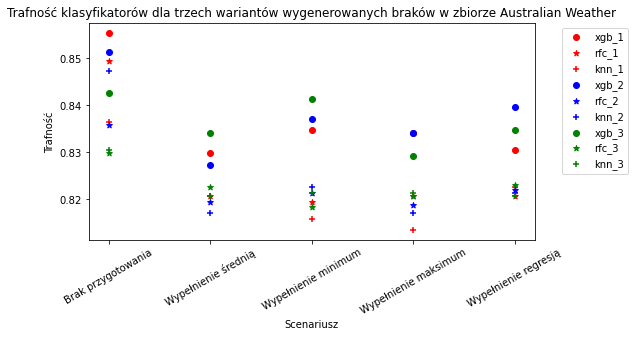
\includegraphics[scale=0.8]{Aus_Weather_Wypełnienie_brakujących}}
        \centering
        \caption{Trafność klasyfikatorów dla trzech wariantów wygenerowanych braków w zbiorze Australian Rain Forecast po wypełnieniu brakujących wartości}
        \end{figure}


Powyżej (Tablica 5.5, Rysunek 5.5) przedstawiono 
trafność klasyfikatorów dla zbioru Australian Rain Forecast, 
po wypełnieniu brakujących wartości w zbiorze.
Dla tego zbioru wypełnienie brakujących wartości w większości
przypadków skutkowało pogorszeniem trafności klasyfikacji, może to 
być spowodowane wielkością zbioru, gdzie pojedyncze braki nie są 
aż tak istotne jak możliwe przekłamania spowodoane uzupełnianiem
braków.

\subsection{Standaryzacja}

\begin{table}[H]
    \begin{tabular}{|l|l|r|r|r|r|r|}
    \hline
    Wariant                                                                                & Scenariusz                                                                                     & \multicolumn{1}{l|}{\begin{tabular}[c]{@{}l@{}}Trafność \\ xgBoost\end{tabular}} & \multicolumn{1}{l|}{\begin{tabular}[c]{@{}l@{}}Trafność\\ Random \\ Forest\end{tabular}} & \multicolumn{1}{l|}{\begin{tabular}[c]{@{}l@{}}Trafność\\ k-najbliższych\\  sąsiadów\end{tabular}} & \multicolumn{1}{l|}{\begin{tabular}[c]{@{}l@{}}Średnia\\ trafność\end{tabular}} & \multicolumn{1}{l|}{\begin{tabular}[c]{@{}l@{}}Błąd \\ standardowy\end{tabular}} \\ \hline
                                                                                           & Brak przygotowania                                                                             & \cellcolor[HTML]{67FD9A}0,8364865                                                & \cellcolor[HTML]{67FD9A}0,8216216                                                        & \cellcolor[HTML]{67FD9A}0,8344595                                                                  & \cellcolor[HTML]{FFCC67}0,8308559                                               & \cellcolor[HTML]{FFCC67}0,004654049171                                           \\ \cline{2-7} 
                                                                                           & Standaryzacja                                                                                  & 0,8334347                                                                        & 0,8206687                                                                                & 0,8206687                                                                                          & 0,8249240                                                                       & 0,004255319149                                                                   \\ \cline{2-7} 
                                                                                           & Skalowanie do (0-1)                                                                            & 0,8334347                                                                        & 0,8206687                                                                                & 0,8164134                                                                                          & 0,8235056                                                                       & 0,005114257128                                                                   \\ \cline{2-7} 
    \multirow{-4}{*}{\begin{tabular}[c]{@{}l@{}}Australian\\ Rain Forecast 1\end{tabular}} & \begin{tabular}[c]{@{}l@{}}Skalowanie (0-1)\\  i usuwanie wartości\\  odstających\end{tabular} & 0,8272446                                                                        & 0,8068111                                                                                & 0,8123839                                                                                          & 0,8154799                                                                       & 0,006098363964                                                                   \\ \hline
                                                                                           & Brak przygotowania                                                                             & \cellcolor[HTML]{67FD9A}0,8418919                                                & 0,8128378                                                                                & \cellcolor[HTML]{67FD9A}0,8243243                                                                  & \cellcolor[HTML]{FFCC67}0,8263514                                               & \cellcolor[HTML]{FFCC67}0,008448197898                                           \\ \cline{2-7} 
                                                                                           & Standaryzacja                                                                                  & 0,8285714                                                                        & \cellcolor[HTML]{67FD9A}0,8206687                                                        & 0,8176292                                                                                          & 0,8222898                                                                       & 0,003261089552                                                                   \\ \cline{2-7} 
                                                                                           & Skalowanie do (0-1)                                                                            & 0,8285714                                                                        & \cellcolor[HTML]{67FD9A}0,8206687                                                        & 0,8121581                                                                                          & 0,8204661                                                                       & 0,004739216034                                                                   \\ \cline{2-7} 
    \multirow{-4}{*}{\begin{tabular}[c]{@{}l@{}}Australian\\ Rain Forecast 2\end{tabular}} & \begin{tabular}[c]{@{}l@{}}Skalowanie (0-1)\\  i usuwanie wartości\\  odstających\end{tabular} & 0,8210526                                                                        & 0,8049536                                                                                & 0,8123839                                                                                          & 0,8127967                                                                       & 0,004651982526                                                                   \\ \hline
                                                                                           & Brak przygotowania                                                                             & \cellcolor[HTML]{67FD9A}0,8581081                                                & \cellcolor[HTML]{67FD9A}0,8405405                                                        & \cellcolor[HTML]{67FD9A}0,8432432                                                                  & \cellcolor[HTML]{FFCC67}0,8472973                                               & \cellcolor[HTML]{FFCC67}0,005461421465                                           \\ \cline{2-7} 
                                                                                           & Standaryzacja                                                                                  & 0,8352584                                                                        & 0,8206687                                                                                & 0,8285714                                                                                          & 0,8281662                                                                       & 0,004216545501                                                                   \\ \cline{2-7} 
                                                                                           & Skalowanie do (0-1)                                                                            & 0,8352584                                                                        & 0,8206687                                                                                & 0,8151976                                                                                          & 0,8237082                                                                       & 0,0059871476                                                                     \\ \cline{2-7} 
    \multirow{-4}{*}{\begin{tabular}[c]{@{}l@{}}Australian\\ Rain Forecast 3\end{tabular}} & \begin{tabular}[c]{@{}l@{}}Skalowanie (0-1)\\  i usuwanie wartości\\  odstających\end{tabular} & 0,8490099                                                                        & 0,8298267                                                                                & 0,8254950                                                                                          & 0,8347772                                                                       & 0,00722536299                                                                    \\ \hline
    \end{tabular}
    \caption{Trafność klasyfikatorów dla zbioru Australian Rain Forecast po scenariuszach związanych z standaryzacją}
    \end{table}

    \begin{figure}[H]
        \centerline{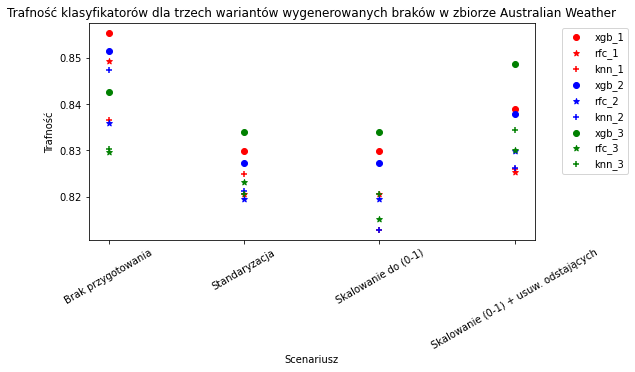
\includegraphics[scale=0.8]{Aus_Weather_Standaryzacja}}
        \centering
        \caption{Trafność klasyfikatorów dla trzech wariantów wygenerowanych braków w zbiorze Australian Rain Forecast po standaryzacji}
        \end{figure}


Powyżej (Tablica 5.6, Rysunek 5.6) przedstawiono 
trafność klasyfikatorów dla zbioru Australian Rain Forecast, 
po scenariuszach związanych ze standaryzacją.
Podobnie jak dla wypełniania brakujących wartości, w większości przypadków
standaryzacja powoduje pogorszenie trafności klasyfikacji

\subsection{Kodowanie}

\begin{table}[H]
    \begin{tabular}{|l|l|r|r|r|r|r|}
    \hline
    Wariant                                                                                & Scenariusz                                                                                                      & \multicolumn{1}{l|}{\begin{tabular}[c]{@{}l@{}}Trafność \\ xgBoost\end{tabular}} & \multicolumn{1}{l|}{\begin{tabular}[c]{@{}l@{}}Trafność\\ Random \\ Forest\end{tabular}} & \multicolumn{1}{l|}{\begin{tabular}[c]{@{}l@{}}Trafność\\ k-najbliższych\\  sąsiadów\end{tabular}} & \multicolumn{1}{l|}{\begin{tabular}[c]{@{}l@{}}Średnia\\ trafność\end{tabular}} & \multicolumn{1}{l|}{\begin{tabular}[c]{@{}l@{}}Błąd \\ standardowy\end{tabular}} \\ \hline
                                                                                           & \begin{tabular}[c]{@{}l@{}}Brak \\ przygotowania\end{tabular}                                                   & 0,8364865                                                                        & 0,8216216                                                                                & 0,8344595                                                                                          & 0,8308559                                                                       & 0,004654049171                                                                   \\ \cline{2-7} 
                                                                                           & \begin{tabular}[c]{@{}l@{}}Kodowanie \\ wartości \\ kateg.\end{tabular}                                         & \cellcolor[HTML]{67FD9A}1,0000000                                                & \cellcolor[HTML]{67FD9A}0,9547297                                                        & \cellcolor[HTML]{67FD9A}0,8391892                                                                  & \cellcolor[HTML]{FFCC67}0,9313063                                               & \cellcolor[HTML]{FFCC67}0,04787665329                                            \\ \cline{2-7} 
    \multirow{-3}{*}{\begin{tabular}[c]{@{}l@{}}Australian\\ Rain Forecast 1\end{tabular}} & \begin{tabular}[c]{@{}l@{}}Kodowanie \\ wartości \\ kateg. i \\ wypełnianie\\ war. brak.\\ średnią\end{tabular} & \cellcolor[HTML]{67FD9A}1,0000000                                                & 0,9428571                                                                                & 0,8255319                                                                                          & 0,9227964                                                                       & 0,05135369075                                                                    \\ \hline
                                                                                           & \begin{tabular}[c]{@{}l@{}}Brak \\ przygotowania\end{tabular}                                                   & 0,8418919                                                                        & 0,8128378                                                                                & 0,8243243                                                                                          & 0,8263514                                                                       & 0,008448197898                                                                   \\ \cline{2-7} 
                                                                                           & \begin{tabular}[c]{@{}l@{}}Kodowanie \\ wartości \\ kategorycznych\end{tabular}                                 & \cellcolor[HTML]{67FD9A}1,0000000                                                & \cellcolor[HTML]{67FD9A}0,9500000                                                        & \cellcolor[HTML]{67FD9A}0,8304054                                                                  & \cellcolor[HTML]{FFCC67}0,9268018                                               & \cellcolor[HTML]{FFCC67}0,05031301663                                            \\ \cline{2-7} 
    \multirow{-3}{*}{\begin{tabular}[c]{@{}l@{}}Australian\\ Rain Forecast 2\end{tabular}} & \begin{tabular}[c]{@{}l@{}}Kodowanie \\ wartości \\ kateg. i \\ wypełnianie\\ war. brak.\\ średnią\end{tabular} & \cellcolor[HTML]{67FD9A}1,0000000                                                & 0,9465046                                                                                & 0,8243161                                                                                          & 0,9236069                                                                       & 0,05199177759                                                                    \\ \hline
                                                                                           & \begin{tabular}[c]{@{}l@{}}Brak \\ przygotowania\end{tabular}                                                   & 0,8581081                                                                        & 0,8405405                                                                                & 0,8432432                                                                                          & 0,8472973                                                                       & 0,005461421465                                                                   \\ \cline{2-7} 
                                                                                           & \begin{tabular}[c]{@{}l@{}}Kodowanie \\ wartości \\ kategorycznych\end{tabular}                                 & \cellcolor[HTML]{67FD9A}1,0000000                                                & \cellcolor[HTML]{67FD9A}0,9635135                                                        & \cellcolor[HTML]{67FD9A}0,8506757                                                                  & \cellcolor[HTML]{FFCC67}0,9380631                                               & \cellcolor[HTML]{FFCC67}0,04494527239                                            \\ \cline{2-7} 
    \multirow{-3}{*}{\begin{tabular}[c]{@{}l@{}}Australian\\ Rain Forecast 3\end{tabular}} & \begin{tabular}[c]{@{}l@{}}Kodowanie \\ wartości \\ kateg. i \\ wypełnianie\\ war. brak.\\ średnią\end{tabular} & \cellcolor[HTML]{67FD9A}1,0000000                                                & 0,9440729                                                                                & 0,8249240                                                                                          & 0,9229990                                                                       & 0,05162681561                                                                    \\ \hline
    \end{tabular}
    \caption{Trafność klasyfikatorów dla zbioru Australian Rain Forecast po scenariuszach związanych z kodowaniem}
    \end{table}


    \begin{figure}[H]
        \centerline{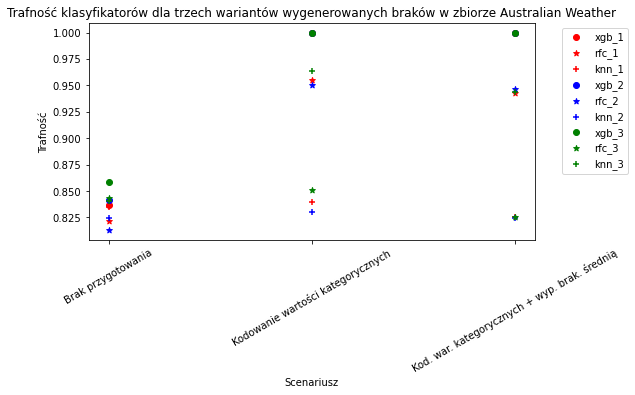
\includegraphics[scale=0.8]{Aus_Weather_Kodowanie}}
        \centering
        \caption{Trafność klasyfikatorów dla trzech wariantów wygenerowanych braków w zbiorze Australian Rain Forecast po kodowaniu wartości kategorycznych}
        \end{figure}

Powyżej (Tablica 5.7, Rysunek 5.7) przedstawiono 
trafność klasyfikatorów dla zbioru Australian Rain Forecast, 
po kodowaniu wartości kategorycznych.
Dopiero kodowanie wartości kategorycznych przyniosło poprawę 
trafności klasyfikacji względem braku przygotowania.
Dla dwóch z klasyfikatorów dodatkowe wypełnienie brakujących wartości 
nie przynosi zwiększenia trafności klasyfikacji.

\subsection{Indywidualne podejście}

\begin{table}[H]
    \begin{tabular}{|l|l|r|r|r|r|r|}
    \hline
    Wariant                                                                                & Scenariusz                                                                      & \multicolumn{1}{l|}{\begin{tabular}[c]{@{}l@{}}Trafność \\ xgBoost\end{tabular}} & \multicolumn{1}{l|}{\begin{tabular}[c]{@{}l@{}}Trafność\\ Random \\ Forest\end{tabular}} & \multicolumn{1}{l|}{\begin{tabular}[c]{@{}l@{}}Trafność\\ k-najbliższych\\  sąsiadów\end{tabular}} & \multicolumn{1}{l|}{\begin{tabular}[c]{@{}l@{}}Średnia\\ trafność\end{tabular}} & \multicolumn{1}{l|}{\begin{tabular}[c]{@{}l@{}}Błąd \\ standardowy\end{tabular}} \\ \hline
                                                                                           & \begin{tabular}[c]{@{}l@{}}Brak \\ przygotowania\end{tabular}                   & 0,8364865                                                                        & 0,8216216                                                                                & \cellcolor[HTML]{67FD9A}0,8344595                                                                  & 0,8308559                                                                       & 0,004654049171                                                                   \\ \cline{2-7} 
    \multirow{-2}{*}{\begin{tabular}[c]{@{}l@{}}Australian\\ Rain Forecast 1\end{tabular}} & \begin{tabular}[c]{@{}l@{}}Przygotowanie\\ dostosowane do\\ zbioru\end{tabular} & \cellcolor[HTML]{67FD9A}1,0000000                                                & \cellcolor[HTML]{67FD9A}0,9796296                                                        & 0,8006173                                                                                          & \cellcolor[HTML]{FFCC67}0,9267490                                               & \cellcolor[HTML]{FFCC67}0,06333940293                                            \\ \hline
                                                                                           & \begin{tabular}[c]{@{}l@{}}Brak \\ przygotowania\end{tabular}                   & 0,8418919                                                                        & 0,8128378                                                                                & \cellcolor[HTML]{67FD9A}0,8243243                                                                  & 0,8263514                                                                       & 0,008448197898                                                                   \\ \cline{2-7} 
    \multirow{-2}{*}{\begin{tabular}[c]{@{}l@{}}Australian\\ Rain Forecast 2\end{tabular}} & \begin{tabular}[c]{@{}l@{}}Przygotowanie\\ dostosowane do\\ zbioru\end{tabular} & \cellcolor[HTML]{67FD9A}1,0000000                                                & \cellcolor[HTML]{67FD9A}0,9833436                                                        & 0,7809994                                                                                          & \cellcolor[HTML]{F8A102}0,9214477                                               & \cellcolor[HTML]{F8A102}0,07038856187                                            \\ \hline
                                                                                           & \begin{tabular}[c]{@{}l@{}}Brak \\ przygotowania\end{tabular}                   & 0,8581081                                                                        & 0,8405405                                                                                & \cellcolor[HTML]{67FD9A}0,8432432                                                                  & 0,8472973                                                                       & 0,005461421465                                                                   \\ \cline{2-7} 
    \multirow{-2}{*}{\begin{tabular}[c]{@{}l@{}}Australian\\ Rain Forecast 3\end{tabular}} & \begin{tabular}[c]{@{}l@{}}Przygotowanie\\ dostosowane do\\ zbioru\end{tabular} & \cellcolor[HTML]{67FD9A}1,0000000                                                & \cellcolor[HTML]{67FD9A}0,9722736                                                        & 0,7997535                                                                                          & \cellcolor[HTML]{FFCC67}0,9240090                                               & \cellcolor[HTML]{FFCC67}0,06264119942                                            \\ \hline
    \end{tabular}
    \caption{Trafność klasyfikatorów dla zbioru Aus Rain Forecast po indywidualnym podejściu do zbioru}
    \end{table}


    \begin{figure}[H]
    \centerline{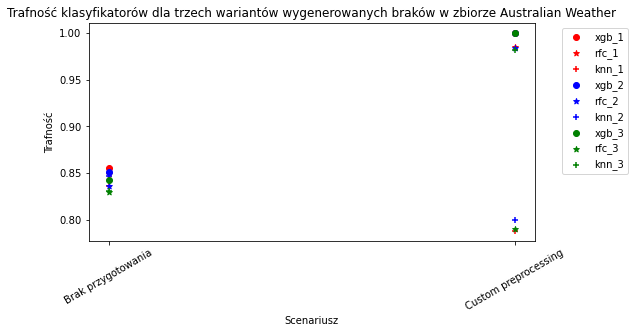
\includegraphics[scale=0.8]{Aus_Weather_Custom}}
    \centering
    \caption{Trafność klasyfikatorów dla trzech wariantów wygenerowanych braków w zbiorze Australian Rain Forecast po indywidualnym podejściu dla zbiorów}
    \end{figure}

Powyżej (Tablica 5.8, Rysunek 5.8) przedstawiono 
trafność klasyfikatorów dla zbioru Australian Rain Forecast, 
po przygotowaniu danych dostosowanych do zbioru.
Dla klasyfikatorów xgBoost i lasu losowego indywidualne podejście 
przyniosło poprawę wyników, natomiast dla k-najbliższych sąsiadów
pogorszyło trafność. Może to być związane z faktem, że częścią przygotowania
w tym scenariuszu było rozbicie kolumny z datą na osobne kolumny dnia, 
miesiąca oraz roku, co mogło szczególnie negatywnie wpłynąć na klasyfikator 
k-najbliższych sąsiadów.

\section{Titanic Survival}



\subsection{Wypełnienie brakujących wartości}


\begin{table}[H]
    \begin{tabular}{|l|l|r|r|r|r|r|}
    \hline
    Wariant                     & Scenariusz           & \multicolumn{1}{l|}{\begin{tabular}[c]{@{}l@{}}Trafność \\ xgBoost\end{tabular}} & \multicolumn{1}{l|}{\begin{tabular}[c]{@{}l@{}}Trafność\\ Random \\ Forest\end{tabular}} & \multicolumn{1}{l|}{\begin{tabular}[c]{@{}l@{}}Trafność\\ k-najbliższych\\  sąsiadów\end{tabular}} & \multicolumn{1}{l|}{\begin{tabular}[c]{@{}l@{}}Średnia\\ trafność\end{tabular}} & \multicolumn{1}{l|}{\begin{tabular}[c]{@{}l@{}}Błąd \\ standardowy\end{tabular}} \\ \hline
                                & Brak przygotowania   & \cellcolor[HTML]{67FD9A}0,7894737                                                & 0,7368421                                                                                & 0,6315789                                                                                          & 0,7192982                                                                       & 0,04641668967                                                                    \\ \cline{2-7} 
                                & Wypełnienie średnią  & 0,7333333                                                                        & 0,7444444                                                                                & \cellcolor[HTML]{67FD9A}0,6888889                                                                  & 0,7222222                                                                       & 0,01697250257                                                                    \\ \cline{2-7} 
                                & Wypełnienie minimum  & 0,7222222                                                                        & 0,7555556                                                                                & \cellcolor[HTML]{67FD9A}0,6888889                                                                  & 0,7222222                                                                       & 0,01924500897                                                                    \\ \cline{2-7} 
                                & Wypełnienie maksimum & 0,6777778                                                                        & 0,7444444                                                                                & 0,6666667                                                                                          & 0,6962963                                                                       & 0,02428680935                                                                    \\ \cline{2-7} 
    \multirow{-5}{*}{Titanic 1} & Wypełnienie regresją & 0,7666667                                                                        & \cellcolor[HTML]{67FD9A}0,7666667                                                        & \cellcolor[HTML]{67FD9A}0,6888889                                                                  & \cellcolor[HTML]{FFCC67}0,7407407                                               & \cellcolor[HTML]{FFCC67}0,02592592593                                            \\ \hline
                                & Brak przygotowania   & 0,5555556                                                                        & 0,6111111                                                                                & 0,5000000                                                                                          & 0,5555556                                                                       & 0,03207501495                                                                    \\ \cline{2-7} 
                                & Wypełnienie średnią  & 0,7444444                                                                        & \cellcolor[HTML]{67FD9A}0,7444444                                                        & \cellcolor[HTML]{67FD9A}0,6888889                                                                  & 0,7259259                                                                       & 0,01851851852                                                                    \\ \cline{2-7} 
                                & Wypełnienie minimum  & 0,7222222                                                                        & 0,7333333                                                                                & 0,6777778                                                                                          & 0,7111111                                                                       & 0,01697250257                                                                    \\ \cline{2-7} 
                                & Wypełnienie maksimum & 0,7111111                                                                        & \cellcolor[HTML]{67FD9A}0,7444444                                                        & 0,6777778                                                                                          & 0,7111111                                                                       & 0,01924500897                                                                    \\ \cline{2-7} 
    \multirow{-5}{*}{Titanic 2} & Wypełnienie regresją & \cellcolor[HTML]{67FD9A}0,7666667                                                & 0,7333333                                                                                & \cellcolor[HTML]{67FD9A}0,6888889                                                                  & \cellcolor[HTML]{FFCC67}0,7296296                                               & \cellcolor[HTML]{FFCC67}0,02252875011                                            \\ \hline
                                & Brak przygotowania   & 0,6315789                                                                        & 0,5263158                                                                                & 0,6842105                                                                                          & 0,6140351                                                                       & 0,04641668967                                                                    \\ \cline{2-7} 
                                & Wypełnienie średnią  & 0,7777778                                                                        & 0,7222222                                                                                & \cellcolor[HTML]{67FD9A}0,6888889                                                                  & \cellcolor[HTML]{FFCC67}0,7296296                                               & \cellcolor[HTML]{FFCC67}0,02592592593                                            \\ \cline{2-7} 
                                & Wypełnienie minimum  & 0,7333333                                                                        & \cellcolor[HTML]{67FD9A}0,7555556                                                        & 0,6666667                                                                                          & 0,7185185                                                                       & 0,02670778723                                                                    \\ \cline{2-7} 
                                & Wypełnienie maksimum & 0,7777778                                                                        & 0,7333333                                                                                & 0,6777778                                                                                          & 0,7296296                                                                       & 0,02892685065                                                                    \\ \cline{2-7} 
    \multirow{-5}{*}{Titanic 3} & Wypełnienie regresją & \cellcolor[HTML]{67FD9A}0,7888889                                                & 0,7333333                                                                                & 0,6777778                                                                                          & 0,7333333                                                                       & 0,03207501495                                                                    \\ \hline
    \end{tabular}
    \caption{Trafność klasyfikatorów dla zbioru Titanic po scenariuszach związanych z wypełnianiem brakujących wartości}
    \end{table}

\begin{figure}[H]
    \centerline{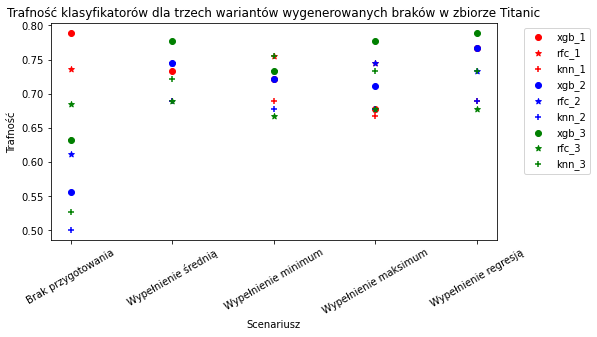
\includegraphics[scale=0.8]{Titanic_Wypełnienie_brakujących}}
    \centering
    \caption{Trafność klasyfikatorów dla trzech wariantów wygenerowanych braków w zbiorze Titanic po wypełnieniu brakujących wartości}
    \end{figure}


Powyżej (Tablica 5.9, Rysunek 5.9) przedstawiono 
trafność klasyfikatorów dla zbioru Titanic, 
po wypełnieniu brakujących wartości w zbiorze.
Dla zdecydowanej większości przypadków wypełnienie brakujących wartości
przynosi zwiększenie trafności klasyfikacji, jednak pomiędzy poszczególnymi przypadkami 
i klasyfikatorami różne wartości, którymi wypełniamy braki przynoszą najlepsze
rezultaty.

\subsection{Standaryzacja}


\begin{table}[H]
    \begin{tabular}{|l|l|r|r|r|r|r|}
    \hline
    Wariant                     & Scenariusz                                                                                     & \multicolumn{1}{l|}{\begin{tabular}[c]{@{}l@{}}Trafność \\ xgBoost\end{tabular}} & \multicolumn{1}{l|}{\begin{tabular}[c]{@{}l@{}}Trafność\\ Random \\ Forest\end{tabular}} & \multicolumn{1}{l|}{\begin{tabular}[c]{@{}l@{}}Trafność\\ k-najbliższych\\  sąsiadów\end{tabular}} & \multicolumn{1}{l|}{\begin{tabular}[c]{@{}l@{}}Średnia\\ trafność\end{tabular}} & \multicolumn{1}{l|}{\begin{tabular}[c]{@{}l@{}}Błąd \\ standardowy\end{tabular}} \\ \hline
                                & \begin{tabular}[c]{@{}l@{}}Brak \\ przygotowania\end{tabular}                                  & \cellcolor[HTML]{67FD9A}0,7894737                                                & 0,7368421                                                                                & 0,6315789                                                                                          & \cellcolor[HTML]{FFCC67}0,7192982                                               & \cellcolor[HTML]{FFCC67}0,04641668967                                            \\ \cline{2-7} 
                                & Standaryzacja                                                                                  & 0,7333333                                                                        & \cellcolor[HTML]{67FD9A}0,7444444                                                        & \cellcolor[HTML]{67FD9A}0,6444444                                                                  & 0,7074074                                                                       & 0,03164445832                                                                    \\ \cline{2-7} 
                                & Skalowanie do (0-1)                                                                            & 0,7333333                                                                        & \cellcolor[HTML]{67FD9A}0,7444444                                                        & 0,5777778                                                                                          & 0,6851852                                                                       & 0,05379940388                                                                    \\ \cline{2-7} 
    \multirow{-4}{*}{Titanic 1} & \begin{tabular}[c]{@{}l@{}}Skalowanie (0-1)\\  i usuwanie wartości\\  odstających\end{tabular} & 0,6093750                                                                        & 0,6406250                                                                                & 0,5625000                                                                                          & 0,6041667                                                                       & 0,02270259866                                                                    \\ \hline
                                & \begin{tabular}[c]{@{}l@{}}Brak \\ przygotowania\end{tabular}                                  & 0,5555556                                                                        & 0,6111111                                                                                & 0,5000000                                                                                          & 0,5555556                                                                       & 0,03207501495                                                                    \\ \cline{2-7} 
                                & Standaryzacja                                                                                  & \cellcolor[HTML]{67FD9A}0,7444444                                                & \cellcolor[HTML]{67FD9A}0,7444444                                                        & \cellcolor[HTML]{67FD9A}0,6444444                                                                  & \cellcolor[HTML]{FFCC67}0,7111111                                               & \cellcolor[HTML]{FFCC67}0,03333333333                                            \\ \cline{2-7} 
                                & Skalowanie do (0-1)                                                                            & \cellcolor[HTML]{67FD9A}0,7444444                                                & \cellcolor[HTML]{67FD9A}0,7444444                                                        & 0,5777778                                                                                          & 0,6888889                                                                       & 0,05555555556                                                                    \\ \cline{2-7} 
    \multirow{-4}{*}{Titanic 2} & \begin{tabular}[c]{@{}l@{}}Skalowanie (0-1)\\  i usuwanie wartości\\  odstających\end{tabular} & 0,6718750                                                                        & 0,6562500                                                                                & 0,5781250                                                                                          & 0,6354167                                                                       & 0,02899877272                                                                    \\ \hline
                                & \begin{tabular}[c]{@{}l@{}}Brak \\ przygotowania\end{tabular}                                  & 0,6315789                                                                        & 0,5263158                                                                                & \cellcolor[HTML]{67FD9A}0,6842105                                                                  & 0,6140351                                                                       & 0,04641668967                                                                    \\ \cline{2-7} 
                                & Standaryzacja                                                                                  & \cellcolor[HTML]{67FD9A}0,7777778                                                & \cellcolor[HTML]{67FD9A}0,7222222                                                        & 0,6333333                                                                                          & \cellcolor[HTML]{FFCC67}0,7111111                                               & \cellcolor[HTML]{FFCC67}0,04206598775                                            \\ \cline{2-7} 
                                & Skalowanie do (0-1)                                                                            & \cellcolor[HTML]{67FD9A}0,7777778                                                & \cellcolor[HTML]{67FD9A}0,7222222                                                        & 0,5777778                                                                                          & 0,6925926                                                                       & 0,05960547015                                                                    \\ \cline{2-7} 
    \multirow{-4}{*}{Titanic 3} & \begin{tabular}[c]{@{}l@{}}Skalowanie (0-1)\\  i usuwanie wartości\\  odstających\end{tabular} & 0,7343750                                                                        & 0,7187500                                                                                & 0,6562500                                                                                          & 0,7031250                                                                       & 0,02386758174                                                                    \\ \hline
    \end{tabular}
    \caption{Trafność klasyfikatorów dla zbioru Titanic po scenariuszach związanych ze standaryzacją}
    \end{table}


\begin{figure}[H]
    \centerline{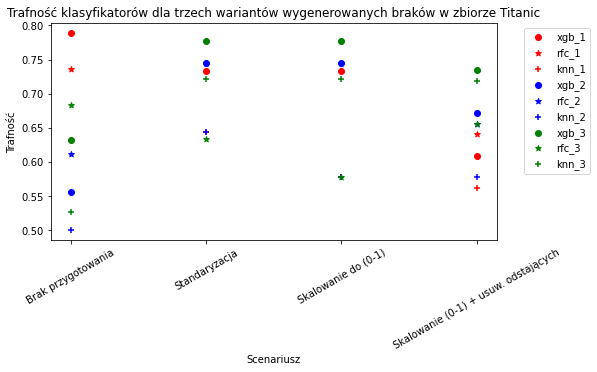
\includegraphics[scale=0.8]{Titanic_Standaryzacja}}
    \centering
    \caption{Trafność klasyfikatorów dla trzech wariantów wygenerowanych braków w zbiorze Titanic po scenariuszach związanych ze standaryzacją}
    \end{figure}


Powyżej (Tablica 5.10, Rysunek 5.10) przedstawiono 
trafność klasyfikatorów dla zbioru Titanic, 
po scenariuszach związanych ze standaryzacją.
Standaryzacja bez skalowania pozwala na uzyskanie 
najlepszych wyników, jednak należy zauważyć, że nie
we wszystkich przypadkach.

\subsection{Kodowanie}

\begin{table}[H]
    \begin{tabular}{|l|l|r|r|r|r|r|}
    \hline
    Wariant                     & Scenariusz                                                                                                      & \multicolumn{1}{l|}{\begin{tabular}[c]{@{}l@{}}Trafność \\ xgBoost\end{tabular}} & \multicolumn{1}{l|}{\begin{tabular}[c]{@{}l@{}}Trafność\\ Random \\ Forest\end{tabular}} & \multicolumn{1}{l|}{\begin{tabular}[c]{@{}l@{}}Trafność\\ k-najbliższych\\  sąsiadów\end{tabular}} & \multicolumn{1}{l|}{\begin{tabular}[c]{@{}l@{}}Średnia\\ trafność\end{tabular}} & \multicolumn{1}{l|}{\begin{tabular}[c]{@{}l@{}}Błąd \\ standardowy\end{tabular}} \\ \hline
                                & \begin{tabular}[c]{@{}l@{}}Brak \\ przygotowania\end{tabular}                                                   & 0,7894737                                                                        & 0,7368421                                                                                & 0,6315789                                                                                          & 0,7192982                                                                       & 0,04641668967                                                                    \\ \cline{2-7} 
                                & \begin{tabular}[c]{@{}l@{}}Kodowanie \\ wartości \\ kateg.\end{tabular}                                         & \cellcolor[HTML]{67FD9A}1,0000000                                                & \cellcolor[HTML]{67FD9A}1,0000000                                                        & 0,5789474                                                                                          & 0,8596491                                                                       & 0,1403508772                                                                     \\ \cline{2-7} 
    \multirow{-3}{*}{Titanic 1} & \begin{tabular}[c]{@{}l@{}}Kodowanie \\ wartości \\ kateg. i \\ wypełnianie\\ war. brak.\\ średnią\end{tabular} & \cellcolor[HTML]{67FD9A}1,0000000                                                & \cellcolor[HTML]{67FD9A}1,0000000                                                        & \cellcolor[HTML]{67FD9A}0,6888889                                                                  & \cellcolor[HTML]{FFCC67}0,8962963                                               & \cellcolor[HTML]{FFCC67}0,1037037037                                             \\ \hline
                                & \begin{tabular}[c]{@{}l@{}}Brak \\ przygotowania\end{tabular}                                                   & 0,5555556                                                                        & 0,6111111                                                                                & 0,5000000                                                                                          & 0,5555556                                                                       & 0,03207501495                                                                    \\ \cline{2-7} 
                                & \begin{tabular}[c]{@{}l@{}}Kodowanie \\ wartości \\ kategorycznych\end{tabular}                                 & \cellcolor[HTML]{67FD9A}1,0000000                                                & \cellcolor[HTML]{67FD9A}1,0000000                                                        & 0,5000000                                                                                          & 0,8333333                                                                       & 0,1666666667                                                                     \\ \cline{2-7} 
    \multirow{-3}{*}{Titanic 2} & \begin{tabular}[c]{@{}l@{}}Kodowanie \\ wartości \\ kateg. i \\ wypełnianie\\ war. brak.\\ średnią\end{tabular} & \cellcolor[HTML]{67FD9A}1,0000000                                                & \cellcolor[HTML]{67FD9A}1,0000000                                                        & \cellcolor[HTML]{67FD9A}0,7000000                                                                  & \cellcolor[HTML]{FFCC67}0,9000000                                               & \cellcolor[HTML]{FFCC67}0,1                                                      \\ \hline
                                & \begin{tabular}[c]{@{}l@{}}Brak \\ przygotowania\end{tabular}                                                   & 0,6315789                                                                        & 0,5263158                                                                                & \cellcolor[HTML]{67FD9A}0,6842105                                                                  & 0,6140351                                                                       & 0,04641668967                                                                    \\ \cline{2-7} 
                                & \begin{tabular}[c]{@{}l@{}}Kodowanie \\ wartości \\ kategorycznych\end{tabular}                                 & \cellcolor[HTML]{67FD9A}1,0000000                                                & \cellcolor[HTML]{67FD9A}1,0000000                                                        & 0,6315789                                                                                          & 0,8771930                                                                       & 0,1228070175                                                                     \\ \cline{2-7} 
    \multirow{-3}{*}{Titanic 3} & \begin{tabular}[c]{@{}l@{}}Kodowanie \\ wartości \\ kateg. i \\ wypełnianie\\ war. brak.\\ średnią\end{tabular} & \cellcolor[HTML]{67FD9A}1,0000000                                                & \cellcolor[HTML]{67FD9A}1,0000000                                                        & 0,6666667                                                                                          & \cellcolor[HTML]{FFCC67}0,8888889                                               & \cellcolor[HTML]{FFCC67}0,1111111111                                             \\ \hline
    \end{tabular}
    \caption{Trafność klasyfikatorów dla zbioru Titanic po scenariuszach związanych z kodowaniem}
    \end{table}


\begin{figure}[H]
    \centerline{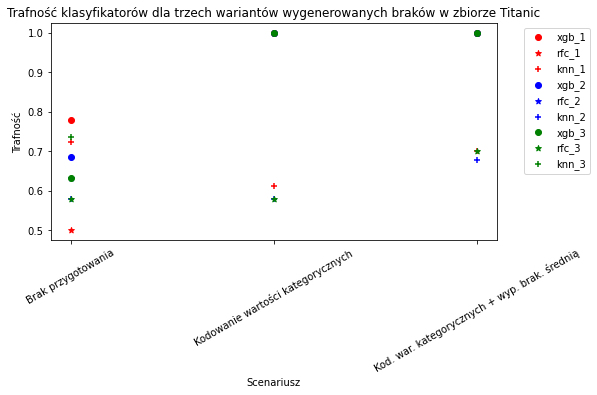
\includegraphics[scale=0.8]{Titanic_Kodowanie}}
    \centering
    \caption{Trafność klasyfikatorów dla trzech wariantów wygenerowanych braków w zbiorze Titanic po scenariuszach związanych ze kodowaniem}
    \end{figure}


Powyżej (Tablica 5.11, Rysunek 5.11) przedstawiono 
trafność klasyfikatorów dla zbioru Titanic, 
po kodowaniu wartości kategorycznych.
Największą trafność klasyfikatory osiągają dla kodowania
wartości oraz wypełniania brakujących wartości średnią.
Dla xgBoost oraz lasu losowego kodowanie pozwala nam uzyskać
100\% trafność klasyfikacji

\subsection{Indywidualne podejście}


\begin{table}[H]
    \begin{tabular}{|l|l|r|r|r|r|r|}
    \hline
    Wariant                     & Scenariusz                                                                      & \multicolumn{1}{l|}{\begin{tabular}[c]{@{}l@{}}Trafność \\ xgBoost\end{tabular}} & \multicolumn{1}{l|}{\begin{tabular}[c]{@{}l@{}}Trafność\\ Random \\ Forest\end{tabular}} & \multicolumn{1}{l|}{\begin{tabular}[c]{@{}l@{}}Trafność\\ k-najbliższych\\  sąsiadów\end{tabular}} & \multicolumn{1}{l|}{\begin{tabular}[c]{@{}l@{}}Średnia\\ trafność\end{tabular}} & \multicolumn{1}{l|}{\begin{tabular}[c]{@{}l@{}}Błąd \\ standardowy\end{tabular}} \\ \hline
                                & \begin{tabular}[c]{@{}l@{}}Brak \\ przygotowania\end{tabular}                   & 0,7894737                                                                        & 0,7368421                                                                                & 0,6315789                                                                                          & 0,7192982                                                                       & 0,04641668967                                                                    \\ \cline{2-7} 
    \multirow{-2}{*}{Titanic 1} & \begin{tabular}[c]{@{}l@{}}Przygotowanie\\ dostosowane do\\ zbioru\end{tabular} & \cellcolor[HTML]{67FD9A}1,0000000                                                & \cellcolor[HTML]{67FD9A}1,0000000                                                        & \cellcolor[HTML]{67FD9A}0,8333333                                                                  & \cellcolor[HTML]{FFCC67}0,9444444                                               & \cellcolor[HTML]{FFCC67}0,05555555556                                            \\ \hline
                                & \begin{tabular}[c]{@{}l@{}}Brak \\ przygotowania\end{tabular}                   & 0,5555556                                                                        & 0,6111111                                                                                & 0,5000000                                                                                          & 0,5555556                                                                       & 0,03207501495                                                                    \\ \cline{2-7} 
    \multirow{-2}{*}{Titanic 2} & \begin{tabular}[c]{@{}l@{}}Przygotowanie\\ dostosowane do\\ zbioru\end{tabular} & \cellcolor[HTML]{67FD9A}1,0000000                                                & \cellcolor[HTML]{67FD9A}1,0000000                                                        & \cellcolor[HTML]{67FD9A}0,8333333                                                                  & \cellcolor[HTML]{FFCC67}0,9444444                                               & \cellcolor[HTML]{FFCC67}0,05555555556                                            \\ \hline
                                & \begin{tabular}[c]{@{}l@{}}Brak \\ przygotowania\end{tabular}                   & 0,6315789                                                                        & 0,5263158                                                                                & 0,6842105                                                                                          & 0,6140351                                                                       & 0,04641668967                                                                    \\ \cline{2-7} 
    \multirow{-2}{*}{Titanic 3} & \begin{tabular}[c]{@{}l@{}}Przygotowanie\\ dostosowane do\\ zbioru\end{tabular} & \cellcolor[HTML]{67FD9A}1,0000000                                                & \cellcolor[HTML]{67FD9A}1,0000000                                                        & \cellcolor[HTML]{67FD9A}0,8222222                                                                  & \cellcolor[HTML]{FFCC67}0,9407407                                               & \cellcolor[HTML]{FFCC67}0,05925925926                                            \\ \hline
    \end{tabular}
    \caption{Trafność klasyfikatorów dla zbioru Titanic po indywidualnym podejściu do zbioru}
    \end{table}

\begin{figure}[H]
    \centerline{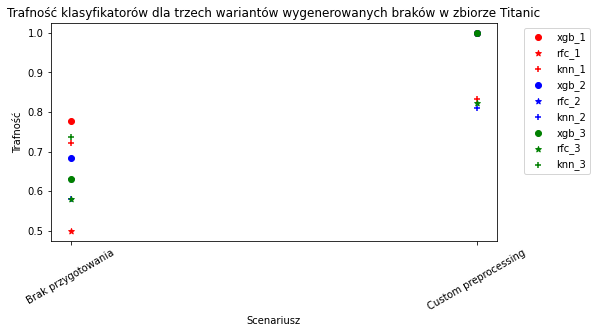
\includegraphics[scale=0.8]{Titanic_Custom}}
    \centering
    \caption{Trafność klasyfikatorów dla trzech wariantów wygenerowanych braków w zbiorze Titanic po indywidualnym podejściu dla zbiorów}
    \end{figure}


Powyżej (Tablica 5.12, Rysunek 5.12) przedstawiono 
trafność klasyfikatorów dla zbioru Titanic, 
po przygotowaniu danych dostosowanym do zbioru.
Dla wszystkich klasyfikatorów dzięki indywidualnemu podejściu
do zbioru uzyskano poprawę trafności klasyfikacji.

\section{Średnie wyniki}

\subsection{Wypełnienie brakujących wartości}

\begin{figure}[H]
    \centerline{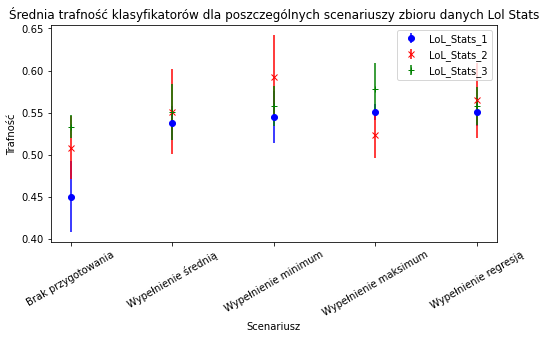
\includegraphics[scale=0.8]{Lol_Stats_Avg_Wypełnienie_brakujących}}
    \centering
    \caption{Średnia trafność klasyfikatorów dla zbioru danych Lol Stats 
    dla grupy scenariuszy wypełniania brakujących wartości}
    \end{figure}

\begin{figure}[H]
    \centerline{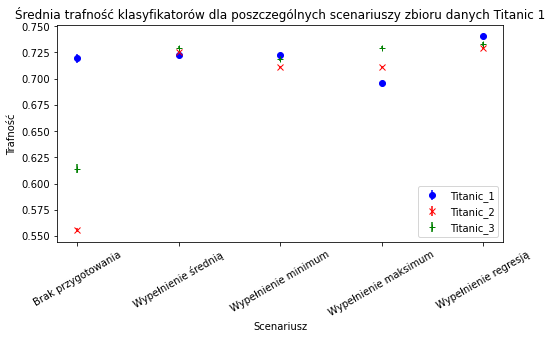
\includegraphics[scale=0.8]{Titanic_Avg_Wypełnienie_brakujących}}
    \centering
    \caption{Średnia trafność klasyfikatorów dla zbioru danych Titanic 
    dla grupy scenariuszy wypełniania brakujących wartości}
    \end{figure}

\begin{figure}[H]
    \centerline{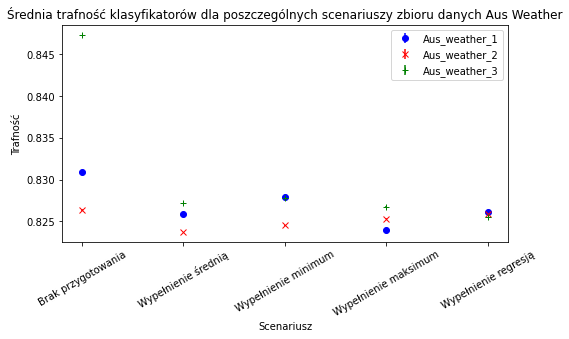
\includegraphics[scale=0.8]{Aus_Weather_Avg_Wypełnienie_brakujących}}
    \centering
    \caption{Średnia trafność klasyfikatorów dla zbioru danych Australian Rain Forecast 
    dla grupy scenariuszy wypełniania brakujących wartości}
    \end{figure}


    Dla Lol Stats oraz Australian Rain Forecast średnia trafność nieznacznie maleje po wypełnieniu brakujących wartości (Rysunek 5.37, Rysunek 5.39). 
    Dla zbioru Titanic w każdym przypadku po wypełnieniu brakujących wartości średnia trafność klasyfikacji wzrosła (Rysunek 5.38)


\subsection{Standaryzacja}

\begin{figure}[H]
    \centerline{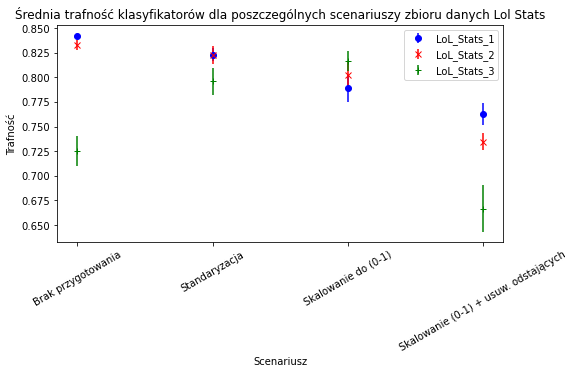
\includegraphics[scale=0.8]{Lol_Stats_Avg_Standaryzacja}}
    \centering
    \caption{Średnia trafność klasyfikatorów dla zbioru danych Lol Stats 
    dla standaryzacji}
    \end{figure}

\begin{figure}[H]
    \centerline{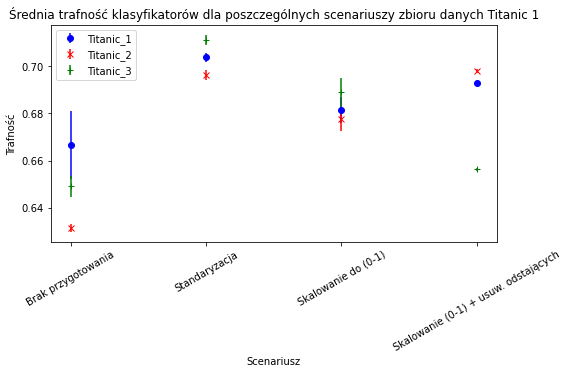
\includegraphics[scale=0.8]{Titanic_Avg_Standaryzacja}}
    \centering
    \caption{Średnia trafność klasyfikatorów dla zbioru danych Titanic 
    dla standaryzacji}
    \end{figure}

\begin{figure}[H]
    \centerline{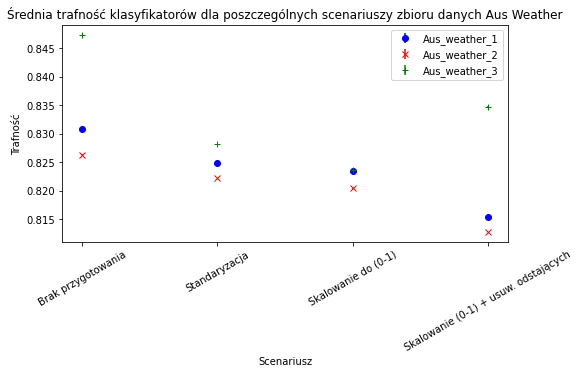
\includegraphics[scale=0.8]{Aus_Weather_Avg_Standaryzacja}}
    \centering
    \caption{Średnia trafność klasyfikatorów dla zbioru danych Australian Rain Forecast 
    dla standaryzacji}
    \end{figure}

    W kwestii Standaryzacji dla zestawu danych Lol Stats 
    najlepszy wynik uzyskujemy dla Standaryzacji oraz 
    Standaryzacji do przedziału (0,1) (Rysunek 5.40), dla 
    Titanic Standaryzacji (Rysunek 5.41), a dla Australian 
    Rain Forecast dla braku przygotowania (Rysunek 5.42)

\subsection{Kodowanie}

\begin{figure}[H]
    \centerline{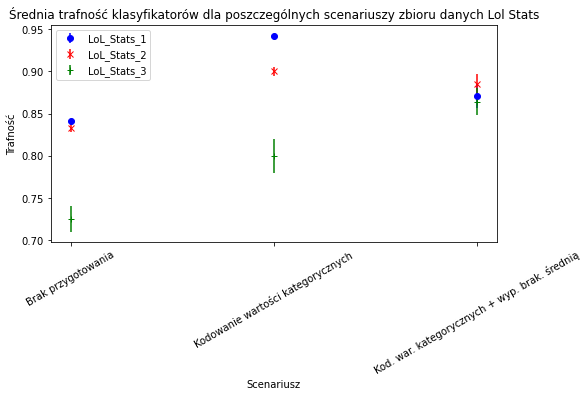
\includegraphics[scale=0.8]{Lol_Stats_Avg_Kodowanie}}
    \centering
    \caption{Średnia trafność klasyfikatorów dla zbioru danych Lol Stats 
    dla kodowania}
    \end{figure}

\begin{figure}[H]
    \centerline{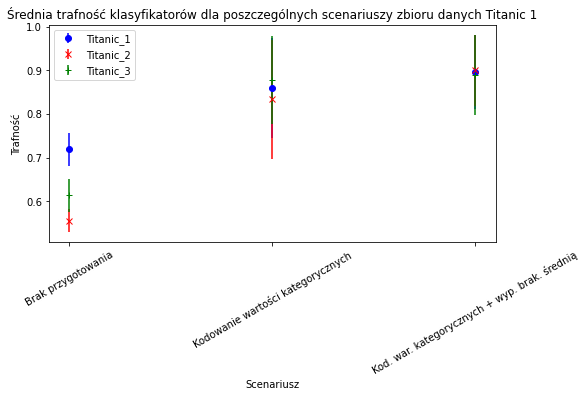
\includegraphics[scale=0.8]{Titanic_Avg_Kodowanie}}
    \centering
    \caption{Średnia trafność klasyfikatorów dla zbioru danych Titanic 
    dla kodowania}
    \end{figure}

\begin{figure}[H]
    \centerline{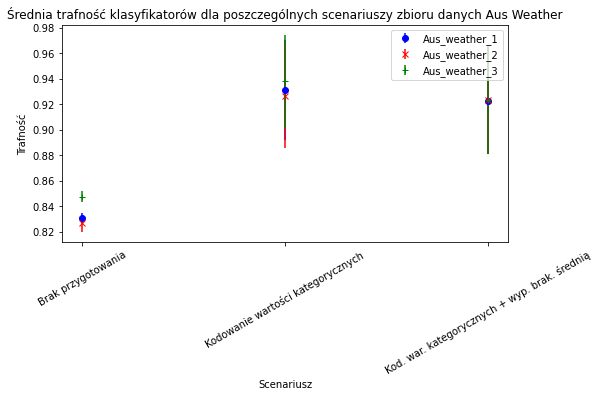
\includegraphics[scale=0.8]{Aus_Weather_Avg_Kodowanie}}
    \centering
    \caption{Średnia trafność klasyfikatorów dla zbioru danych Australian Rain Forecast 
    dla kodowania}
    \end{figure}

    Dla każdego zestawu danych Standaryzacja daje poprawę 
    średniej trafności klasyfikacji, istnieją jednak pewne 
    różnice pomiędzy samym kodowaniem, a kodowaniem z 
    wypełnianiem brakujących wartości. Dla zbioru Lol 
    Stats samo kodowanie powoduje dość rozbieżne wyniki 
    pomiędzy trzema przypadkami wygenerowanych braków, 
    jednak kodowanie z wypełnianiem daje w miarę spójny 
    obraz średniej trafności (Rysunek 5.43), dla Titanic 
    wypełnianie nieznacznie zwiększa średnią trafność 
    klasyfikacji (Rysunek 5.44), natomiast dla Australian Rain Forecast
    najlepszy wynik uzyskujemy dla kodowania bez wypełniania brakujących wartości (Rysunek 5.45)

\subsection{Indywidualne podejście}

\begin{figure}[H]
    \centerline{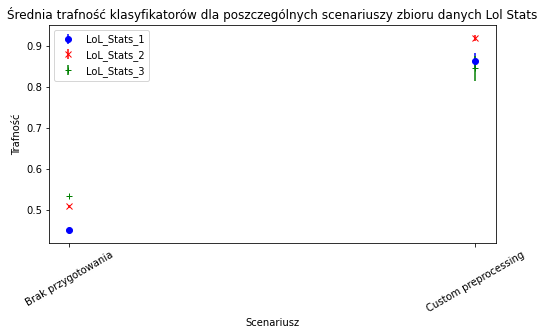
\includegraphics[scale=0.8]{Lol_Stats_Avg_Custom}}
    \centering
    \caption{Średnia trafność klasyfikatorów dla zbioru danych Lol Stats 
    dla indywidualnego podejścia dla zbioru}
    \end{figure}

\begin{figure}[H]
    \centerline{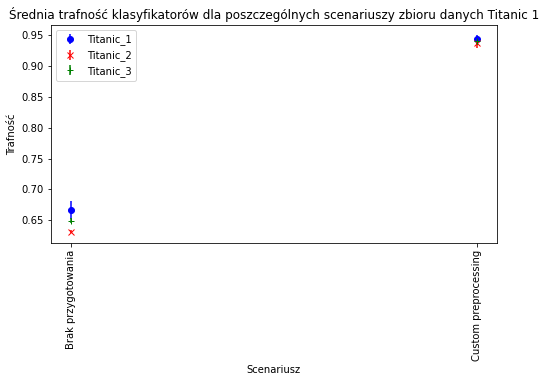
\includegraphics[scale=0.8]{Titanic_Avg_Custom}}
    \centering
    \caption{Średnia trafność klasyfikatorów dla zbioru danych Titanic 
    dla indywidualnego podejścia dla zbioru}
    \end{figure}

\begin{figure}[H]
    \centerline{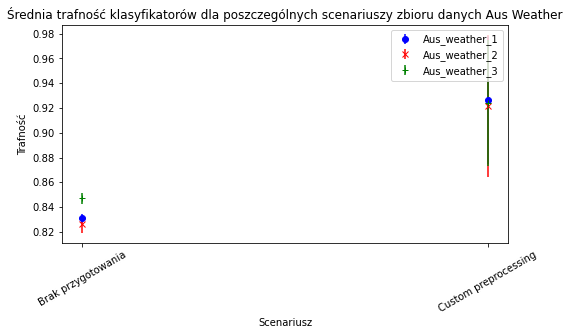
\includegraphics[scale=0.8]{Aus_Weather_Avg_Custom}}
    \centering
    \caption{Średnia trafność klasyfikatorów dla zbioru danych Australian Rain Forecast 
    dla indywidualnego podejścia dla zbioru}
    \end{figure}

    Dla każdego z trzech zbiorów danych podejścia 
    oparte na indywidualnym podejściu do zbioru 
    danych dają wymierną poprawę średniej trafności 
    (Rysunek 5.48, Rysunek 5.47, Rysunek 5.46)


\chapter{Podsumowanie}

W poniższym rozdziale przedstawiono, jak wyniki eksperymentów mają się do założeń postawionych 
przed ich przeprowadzeniem, oraz zapisano wnioski na podstawie wyników.

\section{Konieczność przygotowania danych}

\begin{table}[H]
\begin{tabular}{|l|r|r|r|}
\hline
Wariant                                                               & \multicolumn{1}{l|}{\begin{tabular}[c]{@{}l@{}}Trafność \\ xgBoost\end{tabular}} & \multicolumn{1}{l|}{\begin{tabular}[c]{@{}l@{}}Trafność\\ Random \\ Forest\end{tabular}} & \multicolumn{1}{l|}{\begin{tabular}[c]{@{}l@{}}Trafność\\ k-najbliższych\\  sąsiadów\end{tabular}} \\ \hline
Lol Stats 1                                                           & 0,5500000                                                                        & 0,4250000                                                                                & 0,3750000                                                                                          \\ \hline
Lol Stats 2                                                           & 0,6000000                                                                        & 0,4500000                                                                                & 0,4750000                                                                                          \\ \hline
Lol Stats 3                                                           & 0,5500000                                                                        & 0,5000000                                                                                & 0,5500000                                                                                          \\ \hline
\begin{tabular}[c]{@{}l@{}}Australian\\ Rain Forecast 1\end{tabular}  & 0,8364865                                                                        & 0,8216216                                                                                & 0,8344595                                                                                          \\ \hline
\begin{tabular}[c]{@{}l@{}}Australian \\ Rain Forecast 2\end{tabular} & 0,8418919                                                                        & 0,8128378                                                                                & 0,8243243                                                                                          \\ \hline
\begin{tabular}[c]{@{}l@{}}Australian \\ Rain Forecast 3\end{tabular} & 0,8581081                                                                        & 0,8405405                                                                                & 0,8432432                                                                                          \\ \hline
Titanic 1                                                             & 0,7894737                                                                        & 0,7368421                                                                                & 0,6315789                                                                                          \\ \hline
Titanic 2                                                             & 0,5555556                                                                        & 0,6111111                                                                                & 0,5000000                                                                                          \\ \hline
Titanic 3                                                             & 0,6315789                                                                        & 0,5263158                                                                                & 0,6842105                                                                                          \\ \hline
\end{tabular}
\caption{Trafność klasyfikatorów bez przygotowania danych}
    \end{table}


W zależności od tego, jaki klasyfikator wybierzemy, bez przygotowania danych możemy uzyskać wyniki 
zarówno porównywalne z losowym wyborem klasy, ale i takie, które w wielu przypadkach mogły by być 
uznać za zadowalające (Tablica 6.1). Równocześnie musimy pamiętać, 
że w dziedzinach takich jak medycyna, czy bankowość chcielibyśmy,
aby wytrenowane klasyfikatory były jak najbliższe perfekcji. Z tego powodu cenną informacją jest to,
jak bardzo możemy poprawić trafność klasyfikatorów dzięki przygotowaniu danych.

\section{Wpływ źle dobranych sposobów przygotowania danych}

\begin{table}[H]
\begin{tabular}{|l|l|r|r|r|}
\hline
Wariant                                                                                & Scenariusz                                                                                                   & \multicolumn{1}{l|}{\begin{tabular}[c]{@{}l@{}}Trafność \\ xgBoost\end{tabular}} & \multicolumn{1}{l|}{\begin{tabular}[c]{@{}l@{}}Trafność\\ Random \\ Forest\end{tabular}} & \multicolumn{1}{l|}{\begin{tabular}[c]{@{}l@{}}Trafność\\ k-najbliższych\\  sąsiadów\end{tabular}} \\ \hline
                                                                                       & Brak przygotowania                                                                                           & \multicolumn{1}{l|}{0,8364865}                                                   & \multicolumn{1}{l|}{0,8216216}                                                           & \multicolumn{1}{l|}{0,8344595}                                                                     \\ \cline{2-5} 
\multirow{-2}{*}{\begin{tabular}[c]{@{}l@{}}Australian\\ Rain Forecast 1\end{tabular}} & \begin{tabular}[c]{@{}l@{}}Kodowanie\\ wartości\\ kateg. i\\ wypełnianie\\ war. brak.\\ średnią\end{tabular} & \multicolumn{1}{l|}{\cellcolor[HTML]{FFCCC9}0,8272446}                           & \multicolumn{1}{l|}{\cellcolor[HTML]{FFCCC9}0,8068111}                                   & \multicolumn{1}{l|}{\cellcolor[HTML]{FFCCC9}0,8123839}                                             \\ \hline
                                                                                       & Brak przygotowania                                                                                           & 0,6000000                                                                        & 0,4500000                                                                                & 0,4750000                                                                                          \\ \cline{2-5} 
\multirow{-2}{*}{Lol Stats 2}                                                          & \begin{tabular}[c]{@{}l@{}}Wypełnienie\\ maksimum\end{tabular}                                               & \cellcolor[HTML]{FFCCC9}0,5918367                                                & \cellcolor[HTML]{67FD9A}0,4897959                                                        & \cellcolor[HTML]{67FD9A}0,4897959                                                                  \\ \hline
                                                                                       & Brak przygotowania                                                                                           & 0,7894737                                                                        & 0,7368421                                                                                & 0,6315789                                                                                          \\ \cline{2-5} 
\multirow{-2}{*}{Titanic 1}                                                            & \begin{tabular}[c]{@{}l@{}}Kodowanie \\ wartości \\ kategorycznych\end{tabular}                              & \cellcolor[HTML]{FFCCC9}0,6093750                                                & \cellcolor[HTML]{FFCCC9}0,6406250                                                        & \cellcolor[HTML]{FFCCC9}0,5625000                                                                  \\ \hline
\end{tabular}
\caption{Przykładowe scenariusze dla każdego zbioru danych, w któych przygotowanie danych wpłynęło negatywnie na trafność}
\end{table}

Zgodnie z hipotezą, przygotowanie danych w każdym 
przypadku powinno skutkować lepszymi rezultatami klasyfikacji, jednak podczas eksperymentów 
zauważono przypadki, w których przygotowanie danych pogorszyło jakość klasyfikacji (Tablica 6.2).
Jednoznacznie pokazuje to, że przeprowadzenie przygotowania danych bez
przeanalizowania zbioru i dobrania odpowiednich metod do danego przypadku,
może skutkować pogorszeniem skuteczności klasyfikacji.


\section{Najlepsze wyniki po przygotowaniu danych}

\begin{table}[H]
\begin{tabular}{|l|l|l|l|l|}
\hline
Wariant                    & Scenariusz                                                                                                                 & \begin{tabular}[c]{@{}l@{}}Trafność \\ xgBoost\end{tabular} & \begin{tabular}[c]{@{}l@{}}Trafność\\ Random \\ Forest\end{tabular} & \begin{tabular}[c]{@{}l@{}}Trafność\\ k-najbliższych\\  sąsiadów\end{tabular} \\ \hline
\multirow{3}{*}{Titanic 1} & Brak przygotowania                                                                                                         & 0,7894737                                                   & 0,7368421                                                           & 0,6315789                                                                     \\ \cline{2-5} 
                           & \begin{tabular}[c]{@{}l@{}}Kodowanie \\ wartości \\ kategorycznych\end{tabular}                                            & 1,0000000                                                   & 1,0000000                                                           & 0,6888889                                                                     \\ \cline{2-5} 
                           & \begin{tabular}[c]{@{}l@{}}Przygotowanie \\ dostosowane \\ do zbioru\end{tabular}                                          & 1,0000000                                                   & 1,0000000                                                           & 0,8333333                                                                     \\ \hline
\multirow{3}{*}{Titanic 2} & Brak przygotowania                                                                                                         & 0,5555556                                                   & 0,6111111                                                           & 0,5000000                                                                     \\ \cline{2-5} 
                           & \begin{tabular}[c]{@{}l@{}}Kodowanie wartości\\ kategorycznych i\\ wypełnianie warto±ci\\ brakuj¡cych średnią\end{tabular} & 1,0000000                                                   & 1,0000000                                                           & 0,7000000                                                                     \\ \cline{2-5} 
                           & \begin{tabular}[c]{@{}l@{}}Przygotowanie \\ dostosowane \\ do zbioru\end{tabular}                                          & 1,0000000                                                   & 1,0000000                                                           & 0,8333333                                                                     \\ \hline
\multirow{3}{*}{Titanic 3} & Brak przygotowania                                                                                                         & 0,6315789                                                   & 0,5263158                                                           & 0,6842105                                                                     \\ \cline{2-5} 
                           & Kodowanie wartości kategorycznych                                                                                          & 1,0000000                                                   & 1,0000000                                                           & 0,6666667                                                                     \\ \cline{2-5} 
                           & \begin{tabular}[c]{@{}l@{}}Przygotowanie \\ dostosowane \\ do zbioru\end{tabular}                                          & 1,0000000                                                   & 1,0000000                                                           & 0,8222222                                                                     \\ \hline
\end{tabular}
\caption{Scenariusze dla zbioru Titanic, w któych przygotowanie danych wpłynęło najlepiej na trafność}
\end{table}


Dla zbioru Titanic po przygotowaniu
dwa klasyfikatory osiągają 100\% trafności, 
natomiast w przypadku trzeciego możemy 
zauważyć znaczną poprawę trafności (Tablica 6.3). 
Przed przygotowaniem w poszczególnych przypadkach 
można było zauważyć, że klasyfikator radzi sobie niewiele lepiej 
niż dobierając klasyfikację losowo (50\%), natomiast
po przygotowaniu dostosowanym do danego zbioru, trafność klasyfikacji jest wysoka (80\%), 
bądź nawet perfekcyjna (100\%).


\begin{table}[H]
\begin{tabular}{|l|l|l|l|l|}
\hline
Wariant                      & Scenariusz                                                                                                                 & \begin{tabular}[c]{@{}l@{}}Trafność \\ xgBoost\end{tabular} & \begin{tabular}[c]{@{}l@{}}Trafność\\ Random \\ Forest\end{tabular} & \begin{tabular}[c]{@{}l@{}}Trafność\\ k-najbliższych\\  sąsiadów\end{tabular} \\ \hline
\multirow{3}{*}{Lol Stats 1} & Brak przygotowania                                                                                                         & 0,5500000                                                   & 0,4250000                                                           & 0,3750000                                                                     \\ \cline{2-5} 
                             & \begin{tabular}[c]{@{}l@{}}Kodowanie \\ wartości \\ kategorycznych\end{tabular}                                            & 1,0000000                                                   & 0,8250000                                                           & 0,4500000                                                                     \\ \cline{2-5} 
                             & \begin{tabular}[c]{@{}l@{}}Przygotowanie \\ dostosowane \\ do zbioru\end{tabular}                                          & 1,0000000                                                   & 0,6739130                                                           & 0,9130435                                                                     \\ \hline
\multirow{3}{*}{Lol Stats 2} & Brak przygotowania                                                                                                         & 0,6000000                                                   & 0,4500000                                                           & 0,4750000                                                                     \\ \cline{2-5} 
                             & \begin{tabular}[c]{@{}l@{}}Kodowanie wartości\\ kategorycznych i\\ wypełnianie warto±ci\\ brakuj¡cych średnią\end{tabular} & 0,8418919                                                   & 0,8128378                                                           & 0,8243243                                                                     \\ \cline{2-5} 
                             & \begin{tabular}[c]{@{}l@{}}Przygotowanie \\ dostosowane \\ do zbioru\end{tabular}                                          & 1,0000000                                                   & 0,8000000                                                           & 0,9555556                                                                     \\ \hline
\multirow{3}{*}{Lol Stats 3} & Brak przygotowania                                                                                                         & 0,5500000                                                   & 0,5000000                                                           & 0,5500000                                                                     \\ \cline{2-5} 
                             & Kodowanie wartości kategorycznych                                                                                          & 1,0000000                                                   & 0,8250000                                                           & 0,5250000                                                                     \\ \cline{2-5} 
                             & \begin{tabular}[c]{@{}l@{}}Przygotowanie \\ dostosowane \\ do zbioru\end{tabular}                                          & 1,0000000                                                   & 0,6000000                                                           & 0,9333333                                                                     \\ \hline
\end{tabular}
\caption{Scenariusze dla zbioru Lol Stats, w któych przygotowanie danych wpłynęło najlepiej na trafność}
    \end{table}



    Powyżej przedstawiono najlepsze wyniki klasyfikacji dla zbioru Lol Stats (Tablica 6.4)
    Dla klasyfikatora Random Forest najlepsze wyniki uzyskano przy 
    kodowaniu wartości kategorycznych (około 90\%), dla
    xgBoost zarówno kodowanie jak i indywidualne przygotowanie 
    skutkują idealną klasyfikacją. Dla k-najbliższych sąsiadów najlepsze
    wyniki uzyskano przy indywidualnym podejściu do zbioru (powyżej 90\%)


\begin{table}[H]
\begin{tabular}{|l|l|l|l|l|}
\hline
Wariant                                                                               & Scenariusz                                                                        & \begin{tabular}[c]{@{}l@{}}Trafność \\ xgBoost\end{tabular} & \begin{tabular}[c]{@{}l@{}}Trafność\\ Random \\ Forest\end{tabular} & \begin{tabular}[c]{@{}l@{}}Trafność\\ k-najbliższych\\  sąsiadów\end{tabular} \\ \hline
\multirow{3}{*}{\begin{tabular}[c]{@{}l@{}}Australian\\ Rain Forecast 1\end{tabular}} & Brak przygotowania                                                                & 0,8364865                                                   & 0,8216216                                                           & 0,8344595                                                                     \\ \cline{2-5} 
                                                                                      & \begin{tabular}[c]{@{}l@{}}Kodowanie \\ wartości \\ kategorycznych\end{tabular}   & 1,0000000                                                   & 0,9547297                                                           & 0,8391892                                                                     \\ \cline{2-5} 
                                                                                      & \begin{tabular}[c]{@{}l@{}}Przygotowanie \\ dostosowane \\ do zbioru\end{tabular} & 1,0000000                                                   & 0,9796296                                                           & 0,8006173                                                                     \\ \hline
\multirow{3}{*}{\begin{tabular}[c]{@{}l@{}}Australian\\ Rain Forecast 2\end{tabular}} & Brak przygotowania                                                                & 0,8418919                                                   & 0,8128378                                                           & 0,8243243                                                                     \\ \cline{2-5} 
                                                                                      & \begin{tabular}[c]{@{}l@{}}Kodowanie \\ wartości \\ kategorycznych\end{tabular}   & 1,0000000                                                   & 0,9500000                                                           & 0,8304054                                                                     \\ \cline{2-5} 
                                                                                      & \begin{tabular}[c]{@{}l@{}}Przygotowanie \\ dostosowane \\ do zbioru\end{tabular} & 1,0000000                                                   & 0,9833436                                                           & 0,7809994                                                                     \\ \hline
\multirow{3}{*}{\begin{tabular}[c]{@{}l@{}}Australian\\ Rain Forecast 3\end{tabular}} & Brak przygotowania                                                                & 0,8581081                                                   & 0,8405405                                                           & 0,8432432                                                                     \\ \cline{2-5} 
                                                                                      & \begin{tabular}[c]{@{}l@{}}Kodowanie \\ wartości \\ kategorycznych\end{tabular}   & 1,0000000                                                   & 0,9635135                                                           & 0,8506757                                                                     \\ \cline{2-5} 
                                                                                      & \begin{tabular}[c]{@{}l@{}}Przygotowanie \\ dostosowane \\ do zbioru\end{tabular} & 1,0000000                                                   & 0,9722736                                                           & 0,7997535                                                                     \\ \hline
\end{tabular}
\caption{Scenariusze dla zbioru Australian Rain Forecast, w któych przygotowanie danych wpłynęło najlepiej na trafność}
    \end{table}


    Częścią przygotowania dostosowanego do zbioru 
    Australian Rain Forecast, było rozbicie kolumny z datą na trzy kolumny,
    zawierające dzień, miesiąc oraz rok, co skutkowało pogorszeniem 
    trafności klasyfikacji dla k-najbliższych sąsiadów (Tablica 6.5). 
    Dla pozostałych klasyfikatorów przygotowanie dostosowane do zbioru
    pozwoliło uzyskać najlepszy, bądź jeden z najlepszych wyników. Należy
    zwrócić uwagę na fakt, że różnice w trafności między scenariuszami bez 
    oraz z przygotowaniem danych, nie były tak znaczne jak dla pozostałych zbiorów. 


Tabelka z przykładami
\section{Potencjalne dalsze kierunki badań}
Z wyników eksperymentów wynika korelacja między wielkością zbioru, a 
znaczeniem przygotowania danych. Przy niewielkich zbiorach dzięki przygotowaniu danych
jesteśmy w stanie uzyskać znacznie lepsze wyniki. Natomiast przy większym zbiorze
uzupełnianie braków może prowadzić do przekłamań, a co za tym idzie
mniejszej skuteczności klasyfikatora (Tablica 6.4). Stąd zasadnym były by dalsze badania, 
prowadzone pod kątem zależności między wielkością zbioru, a znaczeniem przygotowania danych.

\section{Najlepsze praktyki przygotowania danych}

Z przeprowadzonych eksperymentów wynika, 
że odpowiednie przygotowanie danych zwiększa w umiarkowanym stopniu celność 
klasyfikatorów. Jeżeli przed analizą danych dogłębnie poznamy i zrozumiemy zbiór danych,
będziemy mogli wybrać najbardziej odpowiednie metody przygotowania danych dla danego zbioru,
a co za tym idzie wyniki analizy będą najbardziej trafne.
Należy jednak zwrócić uwagę, że nie wszystkie 
scenariusze skutkowały jednoznaczną poprawą rezultatów, dlatego dobrą praktyką jest
wieloktorne przygotowywanie danych na różne sposoby tak, aby znaleźć taki, który zwraca najlepsze rezultaty 
Na szczególne wyróżenienie zasługuje kodowanie wartości 
kategorycznych na liczbowe, gdyż w każdym przypadku zastosowanie 
tej metody znacznie zwiększyło trafność klasyfikacji

\begin{thebibliography}{9}
    
    \bibitem{titanic_dataset}
    \href{https://www.kaggle.com/competitions/titanic/data?select=train.csv}{Zbiór danych Titanic dostępny do pobrania ze strony kaggle.com}
    
    \bibitem{lol_stats_dataset}
    \href{https://www.kaggle.com/datasets/vivovinco/league-of-legends-stats-s13}{Zbiór danych Lol Stats dostępny do pobrania ze strony kaggle.com}
    
    \bibitem{australian_rain_dataset}
    \href{https://www.kaggle.com/datasets/jsphyg/weather-dataset-rattle-package}{Zbiór danych Australian Rain dostępny do pobrania ze strony kaggle.com}
    
    \bibitem{data_analysis_def}
    "Transforming Unstructured Data into Useful Information", \emph{Big Data, Mining, and Analytics}, Auerbach Publications, pp. 227–246, 2014-03-12, doi:10.1201/b16666-14, ISBN 978-0-429-09529-0

    \bibitem{data_from_sensors}
    MOIS, George; FOLEA, Silviu; SANISLAV, Teodora. Analysis of three IoT-based wireless sensors for environmental monitoring. \emph{IEEE Transactions on Instrumentation and Measurement}, 2017, 66.8: 2056-2064.
    
    \bibitem{data_from_statistics}
    Margo, Robert A. (2000). \emph{Wages and labor markets in the United States, 1820-1860.} University of Chicago Press. ISBN 0-226-50507-3. OCLC 41285104

    \bibitem{data_from_questionaire}
    Marshall, G. (2005). The purpose, design and administration of a questionnaire for data collection. Radiography, 11(2), 131-136.

    \bibitem{data_from_behavior}
    Fabijan, A., Olsson, H. H., Bosch, J. (2015). Customer feedback and data collection techniques in software R\&D: a literature review. In Software Business: 6th International Conference, ICSOB 2015, Braga, Portugal, June 10-12, 2015, Proceedings 6 (pp. 139-153). Springer International Publishing.

    \bibitem{missing_values}
    Hasan, M. K., Alam, M. A., Roy, S., Dutta, A., Jawad, M. T.,  Das, S. (2021). Missing value imputation affects the performance of machine learning: A review and analysis of the literature (2010–2021). Informatics in Medicine Unlocked, 27, 100799.

    \bibitem{standard_score}
    E. Kreyszig (1979). Advanced Engineering Mathematics (4th ed.). Wiley. p. 880, eq. 5. ISBN 0-471-02140-7.

    \bibitem{one_hot_encoding}
    Okada, S., Ohzeki, M., Taguchi, S. (2019). Efficient partition of integer optimization problems with one-hot encoding. Scientific reports, 9(1), 13036.
    
    \bibitem{outlier_detection}
    Wang, H., Bah, M. J., Hammad, M. (2019). Progress in outlier detection techniques: A survey. Ieee Access, 7, 107964-108000.

    \bibitem{local_outlier_factor}
    Alghushairy, O., Alsini, R., Soule, T., Ma, X. (2020). A review of local outlier factor algorithms for outlier detection in big data streams. Big Data and Cognitive Computing, 5(1), 1.
    
    \bibitem{enconding}
    Potdar, K., Pardawala, T. S., Pai, C. D. (2017). A comparative study of categorical variable encoding techniques for neural network classifiers. International journal of computer applications, 175(4), 7-9.

    \bibitem{classifiers}
    Narudin, F. A., Feizollah, A., Anuar, N. B., Gani, A. (2016). Evaluation of machine learning classifiers for mobile malware detection. Soft Computing, 20, 343-357.
    
    \bibitem{recomendation_systems}
    Khanal, S. S., Prasad, P. W. C., Alsadoon, A., Maag, A. (2020). A systematic review: machine learning based recommendation systems for e-learning. Education and Information Technologies, 25, 2635-2664.

    \bibitem{clustering}
    Ezugwu, A. E., Ikotun, A. M., Oyelade, O. O., Abualigah, L., Agushaka, J. O., Eke, C. I.,  Akinyelu, A. A. (2022). A comprehensive survey of clustering algorithms: State-of-the-art machine learning applications, taxonomy, challenges, and future research prospects. Engineering Applications of Artificial Intelligence, 110, 104743.
    
    \bibitem{decisions_healthcare}
    Sousa, M. J., Pesqueira, A. M., Lemos, C., Sousa, M., \& Rocha, Á. (2019). Decision-making based on big data analytics for people management in healthcare organizations. Journal of medical systems, 43, 1-10.

    \bibitem{decisions_education}
    Schildkamp, K., Lai, M. K., \& Earl, L. (Eds.). (2012). Data-based decision making in education: Challenges and opportunities.

    \bibitem{decsision_buisness}
    Fávero, L. P., \& Belfiore, P. (2019). Data science for business and decision making. Academic Press.

    \bibitem{xgBoost}
    \href{https://xgboost.readthedocs.io/en/stable/}{Definicja dostępna w dokumentacji biblioteki XGBoost}

    \bibitem{k-nearest neighbors}
    Cover, Thomas M.; Hart, Peter E. (1967). "Nearest neighbor pattern classification" (PDF). IEEE Transactions on Information Theory. 13 (1): 21–27. CiteSeerX 10.1.1.68.2616. doi:10.1109/TIT.1967.1053964.

    \bibitem{random forest}
    Ho, Tin Kam (1995). Random Decision Forests (PDF). Proceedings of the 3rd International Conference on Document Analysis and Recognition, Montreal, QC, 14–16 August 1995. pp. 278–282.

    \bibitem{data_quality}
    \href{https://www.ibm.com/topics/data-quality}{Artykuł na temat jakości danych na stronie firmy IBM}
    

\end{thebibliography}

    

\end{document}